\documentclass[10pt, aspectratio=169]{beamer}

% --- Typography & Colors ---
\usefonttheme[onlymath]{serif} % Professional serif math fonts
\usepackage[sfdefault]{plex-sans}
\usepackage[T1]{fontenc}
\usepackage[utf8]{inputenc}
\usepackage{booktabs}
\usepackage{animate}
\usepackage{tikz}
\usepackage{amsmath, amssymb, mathtools}
\usepackage{fontawesome5}
\usetikzlibrary{arrows.meta, shapes.geometric, positioning}

\definecolor{AcademicNavy}{RGB}{0, 51, 102}
\definecolor{SecondaryTitle}{RGB}{153, 0, 0}
\definecolor{SteelBlue}{RGB}{0, 112, 192}
\setbeamercolor{titlelike}{fg=AcademicNavy}
\setbeamercolor{structure}{fg=AcademicNavy}
\setbeamercolor{block title}{fg=SecondaryTitle}

% --- Font Settings ---
\setbeamerfont{frametitle}{size=\Large, series=\bfseries}
\setbeamerfont{block title}{series=\bfseries}

% --- Footer & Page Numbering ---
\setbeamertemplate{navigation symbols}{}
\setbeamerfont{footline}{size=\fontsize{6}{7}\selectfont}
\setbeamercolor{footline}{fg=AcademicNavy!60}
\setbeamertemplate{footline}{
    \hfill
    \insertframenumber / \inserttotalframenumber
    \hspace{0.5cm}\vspace{0.1cm}
}
\setbeamertemplate{itemize items}[circle]

% --- Custom Title Page Design ---
\setbeamertemplate{title page}{
    \vspace*{0.5cm}
    % 1. TOP Logo Header
    \begin{columns}[c, totalwidth=\textwidth]
        \column{0.20\textwidth}
            \raggedright
\includegraphics[height=1.0cm]{LOGO_CNRS_BLEU.png}
        \column{0.60\textwidth}
            \centering
\includegraphics[height=1.0cm]{logo_lspm.png}
        \column{0.20\textwidth}
            \raggedleft
\includegraphics[height=1.0cm]{USPN.png}
    \end{columns}

    \vspace{0.8cm}

    % 2. Title and Subtitle Block
    \begin{centering}
        {\usebeamerfont{title} \usebeamercolor[fg]{title} \huge \textbf{\inserttitle} \par}
        \vspace{0.4cm}
        {\usebeamerfont{subtitle} \usebeamercolor[fg]{subtitle} \small \textit{\insertsubtitle} \par}

        \vspace{0.6cm}

        {\usebeamerfont{author} \large \textbf{\insertauthor} \par}
        \vspace{0.15cm}
        {\usebeamerfont{institute} \small \insertinstitute \par}
        \vspace{0.1cm}
        {\usebeamerfont{date} \scriptsize \insertdate \par}
    \end{centering}

    \vspace{0.6cm}

    % 3. Decorative rule
    \begin{center}
        \textcolor{AcademicNavy!40}{\rule{0.6\textwidth}{0.4pt}}
    \end{center}

    \vspace{0.2cm}

    % 4. Position / affiliation footer
    \begin{center}
        {\tiny \color{AcademicNavy!70}
        Chargé de Recherche CNRS (Section 11) \quad\textbullet\quad
        LSPM-UPR3407, Université Sorbonne Paris Nord \quad\textbullet\quad
        \faEnvelope\ oguzumut.salman@cnrs.fr}
    \end{center}
}

% --- Metadata ---
\title{Decoding Material Intermittency:\\ From Noise to Control}
\subtitle{Harnessing Critical Fluctuations in the Non-Convex Energy Landscapes of Crystals and Metamaterials}
\author{O\u{g}uz Umut SALMAN}
\institute{Laboratoire des Sciences des Procédés et des Matériaux (LSPM) \\ CNRS UPR 3407 $|$ Université Sorbonne Paris Nord}
\date{8 April 2026}

\begin{document}

% Slide 1
\begin{frame}[plain]
    \titlepage
\end{frame}

% --- CV entry helpers (logo + text, mimicking temp.cls) ---
\newcommand{\cvWorkEntry}[5]{%
    % #1=institution  #2=dates  #3=role  #4=description  #5=logo
    \begin{minipage}[c]{0.09\linewidth}
        \includegraphics[width=0.65cm,height=0.65cm,keepaspectratio]{#5}
    \end{minipage}%
    \begin{minipage}[c]{0.89\linewidth}
        {\tiny \color{AcademicNavy}\bfseries\MakeUppercase{#1}},
        {\tiny \color{AcademicNavy}\textit{#3}}
        \hfill
        {\tiny \color{AcademicNavy!70} #2}\\[-0.1cm]
        {\tiny \color{black!70} #4}
    \end{minipage}%
}
\newcommand{\cvEduEntry}[4]{%
    % #1=degree  #2=dates  #3=institution  #4=logo
    \begin{minipage}[c]{0.09\linewidth}
        \includegraphics[width=0.65cm,height=0.65cm,keepaspectratio]{#4}
    \end{minipage}%
    \begin{minipage}[c]{0.89\linewidth}
        {\tiny \color{AcademicNavy}\bfseries\MakeUppercase{#1}}
        \hfill
        {\tiny \color{AcademicNavy!70} #2}\\[-0.1cm]
        {\tiny \color{black!70}\textit{#3}}
    \end{minipage}%
}

% Slide 2: Curriculum Vitae
\begin{frame}{Curriculum Vitae}
\vspace*{0.1cm}

    %% Professional Experience
    {\scriptsize \color{SteelBlue}\textbf{PROFESSIONAL EXPERIENCE}}\\[-0.2cm]
    \textcolor{AcademicNavy!30}{\rule{\linewidth}{0.4pt}}\\[0.04cm]
    %
    \cvWorkEntry{CNRS}{01.2015 – present}{Chargé de recherche}{%
        Researcher – LSPM UPR3407, Université Sorbonne Paris Nord, France. Lecturer – Université Sorbonne Paris Nord.}{LOGO_CNRS_BLEU.png}\\[0.06cm]
    \cvWorkEntry{CNR-IENI}{09.2013 – 09.2015}{Scientific researcher}{%
        Post-Doctoral Fellow – CNR-IENI Milano, Italy. ERC Advanced Grant: Size Effects in Fracture and Plasticity.}{ieni2.png}\\[0.06cm]
    \cvWorkEntry{Harvard University}{10.2012 – 09.2013}{Post-doc}{%
        Post-Doctoral Fellow – Aizenberg Biomineralization \& Biomimetic Laboratory, USA.}{harvard.png}\\[0.06cm]
    \cvWorkEntry{Boğaziçi University}{10.2011 – 10.2012}{Post-doc}{%
        Post-Doctoral Fellow – Physics Department, under supervision of M. Mungan.}{bos.png}\\[0.06cm]
    \cvWorkEntry{École Polytechnique}{06.2009 – 10.2011}{Post-doc}{%
        Post-Doctoral Fellow – Solid Mechanics Laboratory (LMS), Palaiseau, France.}{ept.jpg}

    \vspace{0.25cm}

    %% Education
    {\scriptsize \color{SteelBlue}\textbf{EDUCATION}}\\[-0.2cm]
    \textcolor{AcademicNavy!30}{\rule{\linewidth}{0.4pt}}\\[0.04cm]
    %
    \cvEduEntry{HDR – Mechanics of Displacive Instabilities in Solids}{31 March 2026}{%
        Université Sorbonne Paris Nord, France.}{USPN.png}\\[0.18cm]
    \cvEduEntry{PhD in Physics}{09.2005 – 06.2009}{%
        Université Pierre et Marie Curie, Paris, France \textit{(High Honour Mention).}}{sor.png}\\[0.06cm]
    \cvEduEntry{MSc in Materials Science and Nano-Objects}{09.2004 – 09.2005}{%
        École Polytechnique, Palaiseau, France \textit{(High Honour Mention).}}{ept.jpg}\\[0.06cm]
    \cvEduEntry{BS in Physics}{09.2000 – 06.2004}{%
        Istanbul Technical University, Istanbul, Turkey \textit{(Honour List).}}{itu.png}

\end{frame}

% ===========================================================
% Slide 3: Research Axes — Displacive Phenomena
% ===========================================================
\begin{frame}{Main Research Axes}
\vspace*{-0.15cm}

\vspace{1cm}

% ---- Three pillars ----
\begin{columns}[T, totalwidth=\textwidth]

    %% Phase Transitions
    \column{0.31\textwidth}
    
\begin{tikzpicture}
        \node[rounded corners=4pt, fill=SecondaryTitle, text=white,
              minimum width=\linewidth, minimum height=0.55cm,
              font=\small\bfseries, inner sep=0pt] {Phase Transitions};
    \end{tikzpicture}\\[0.15cm]
    \centering
    {\scriptsize
    \begin{itemize}\setlength\itemsep{0.06cm}
        \item[\color{SteelBlue}\faAngleRight] Reversible martensitic (SMA)
        \item[\color{SteelBlue}\faAngleRight] Reconstructive (Ti, Zr)
        \item[\color{SteelBlue}\faAngleRight] Lattice-invariant shears
    \end{itemize}}

    %% Plasticity
    \column{0.31\textwidth}
    
\begin{tikzpicture}
        \node[rounded corners=4pt, fill=AcademicNavy, text=white,
              minimum width=\linewidth, minimum height=0.55cm,
              font=\small\bfseries, inner sep=0pt] {Plasticity};
    \end{tikzpicture}\\[0.15cm]
    \centering
    {\scriptsize
    \begin{itemize}\setlength\itemsep{0.06cm}
        \item[\color{SteelBlue}\faAngleRight] Dislocation nucleation
        \item[\color{SteelBlue}\faAngleRight] Avalanche dynamics
        \item[\color{SteelBlue}\faAngleRight] Jerky flow \& AE
    \end{itemize}}

    %% Fracture
    \column{0.31\textwidth}
    
\begin{tikzpicture}
        \node[rounded corners=4pt, fill=SteelBlue, text=white,
              minimum width=\linewidth, minimum height=0.55cm,
              font=\small\bfseries, inner sep=0pt] {Fracture};
    \end{tikzpicture}\\[0.15cm]
    \centering
    {\scriptsize
    \begin{itemize}\setlength\itemsep{0.06cm}
        \item[\color{SteelBlue}\faAngleRight] Crack nucleation/propagation in thin films
        \item[\color{SteelBlue}\faAngleRight] Pattern formation
    \end{itemize}}

\end{columns}

\vspace{0.15cm}

% ---- Three images matching column order ----
\begin{columns}[c, totalwidth=\textwidth]
    \column{0.31\textwidth}
    \centering
    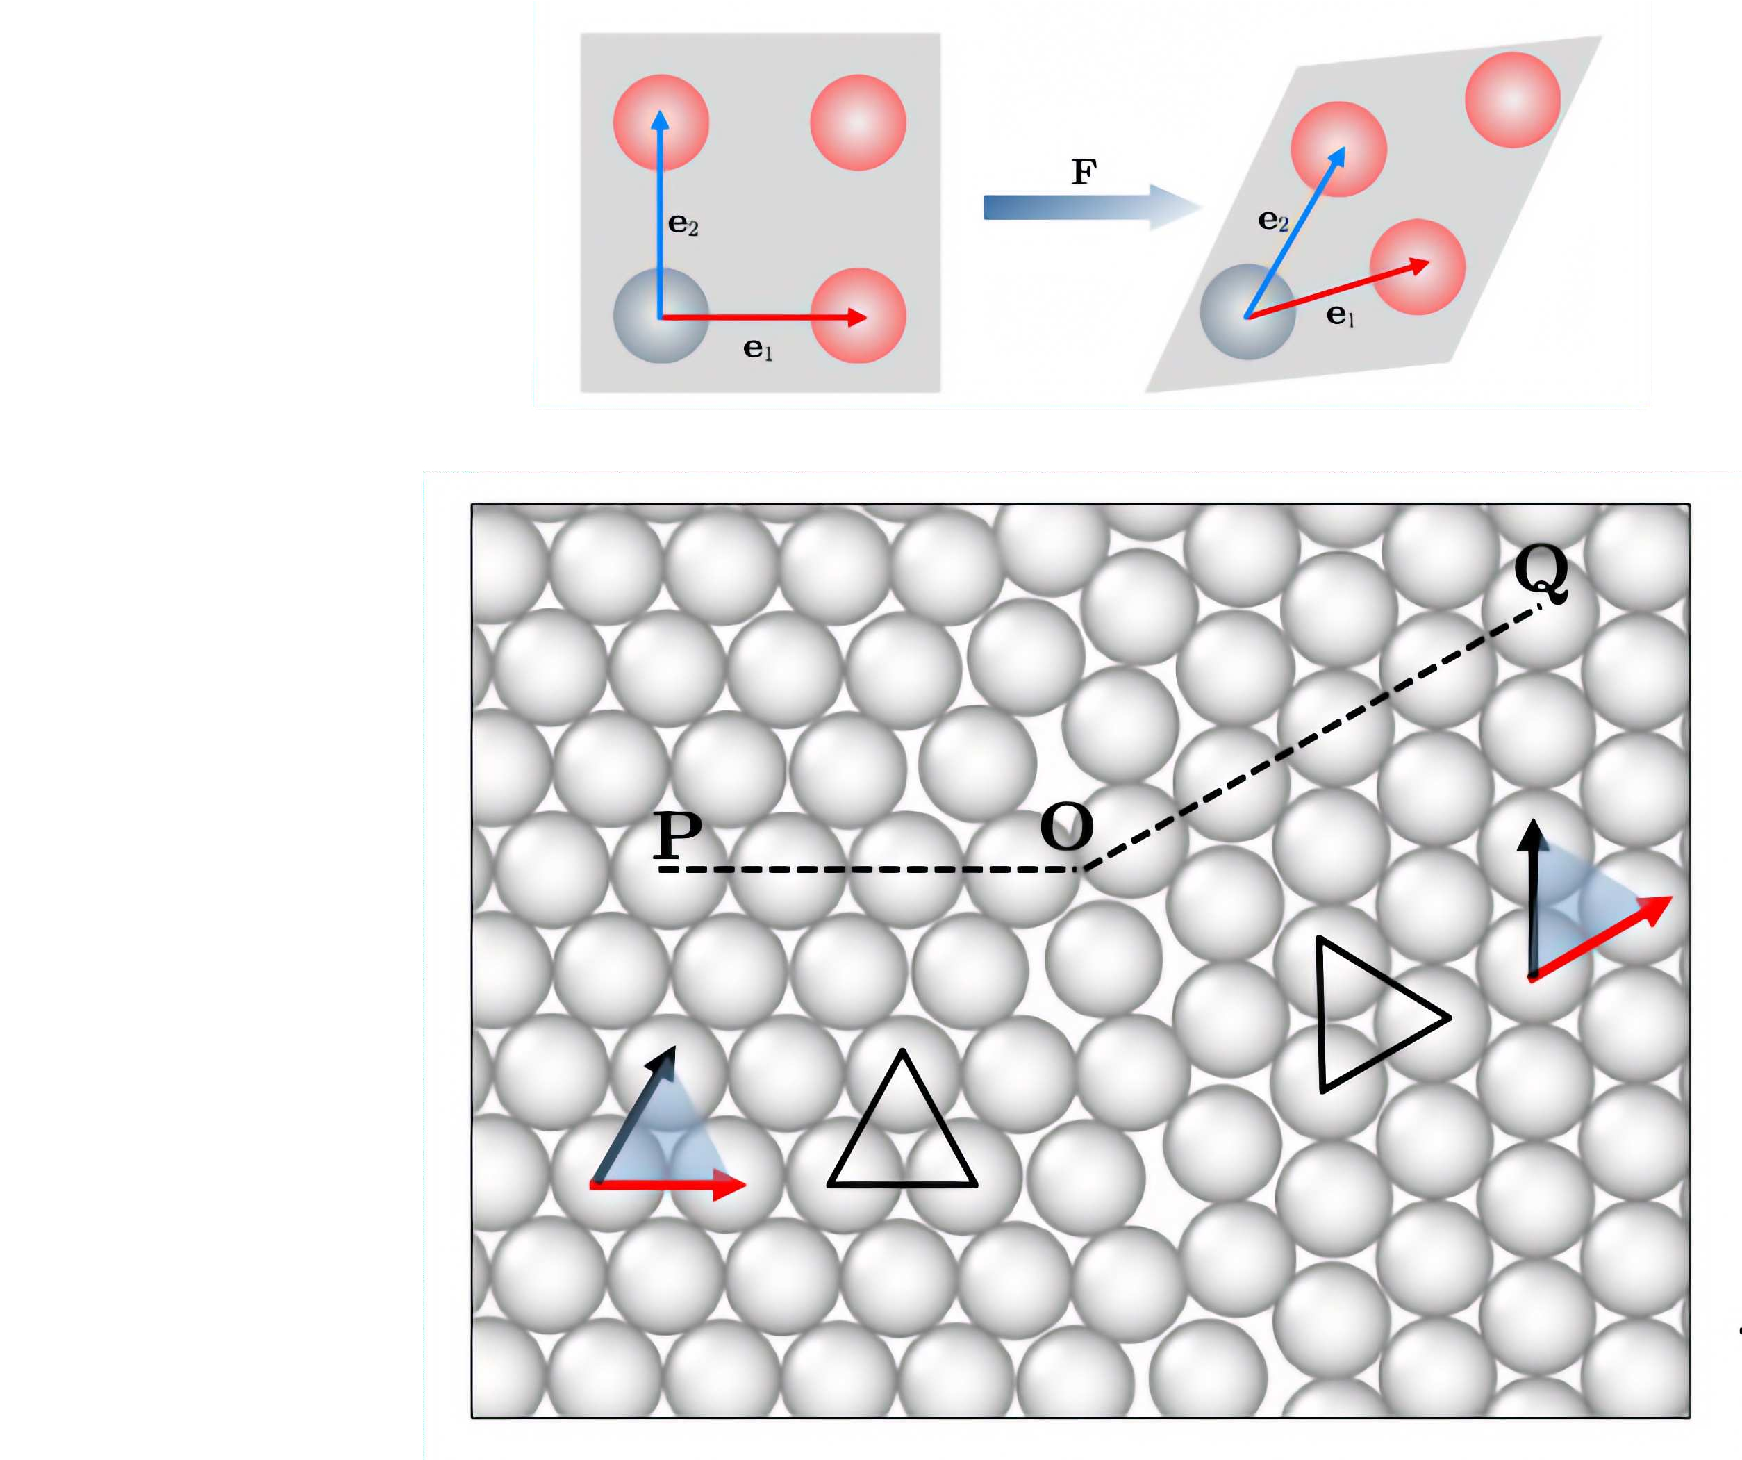
\includegraphics[width=0.9\linewidth, height=2.8cm, keepaspectratio]{figures_dr/fig_phasetrans.pdf}

    \column{0.31\textwidth}
    \centering
    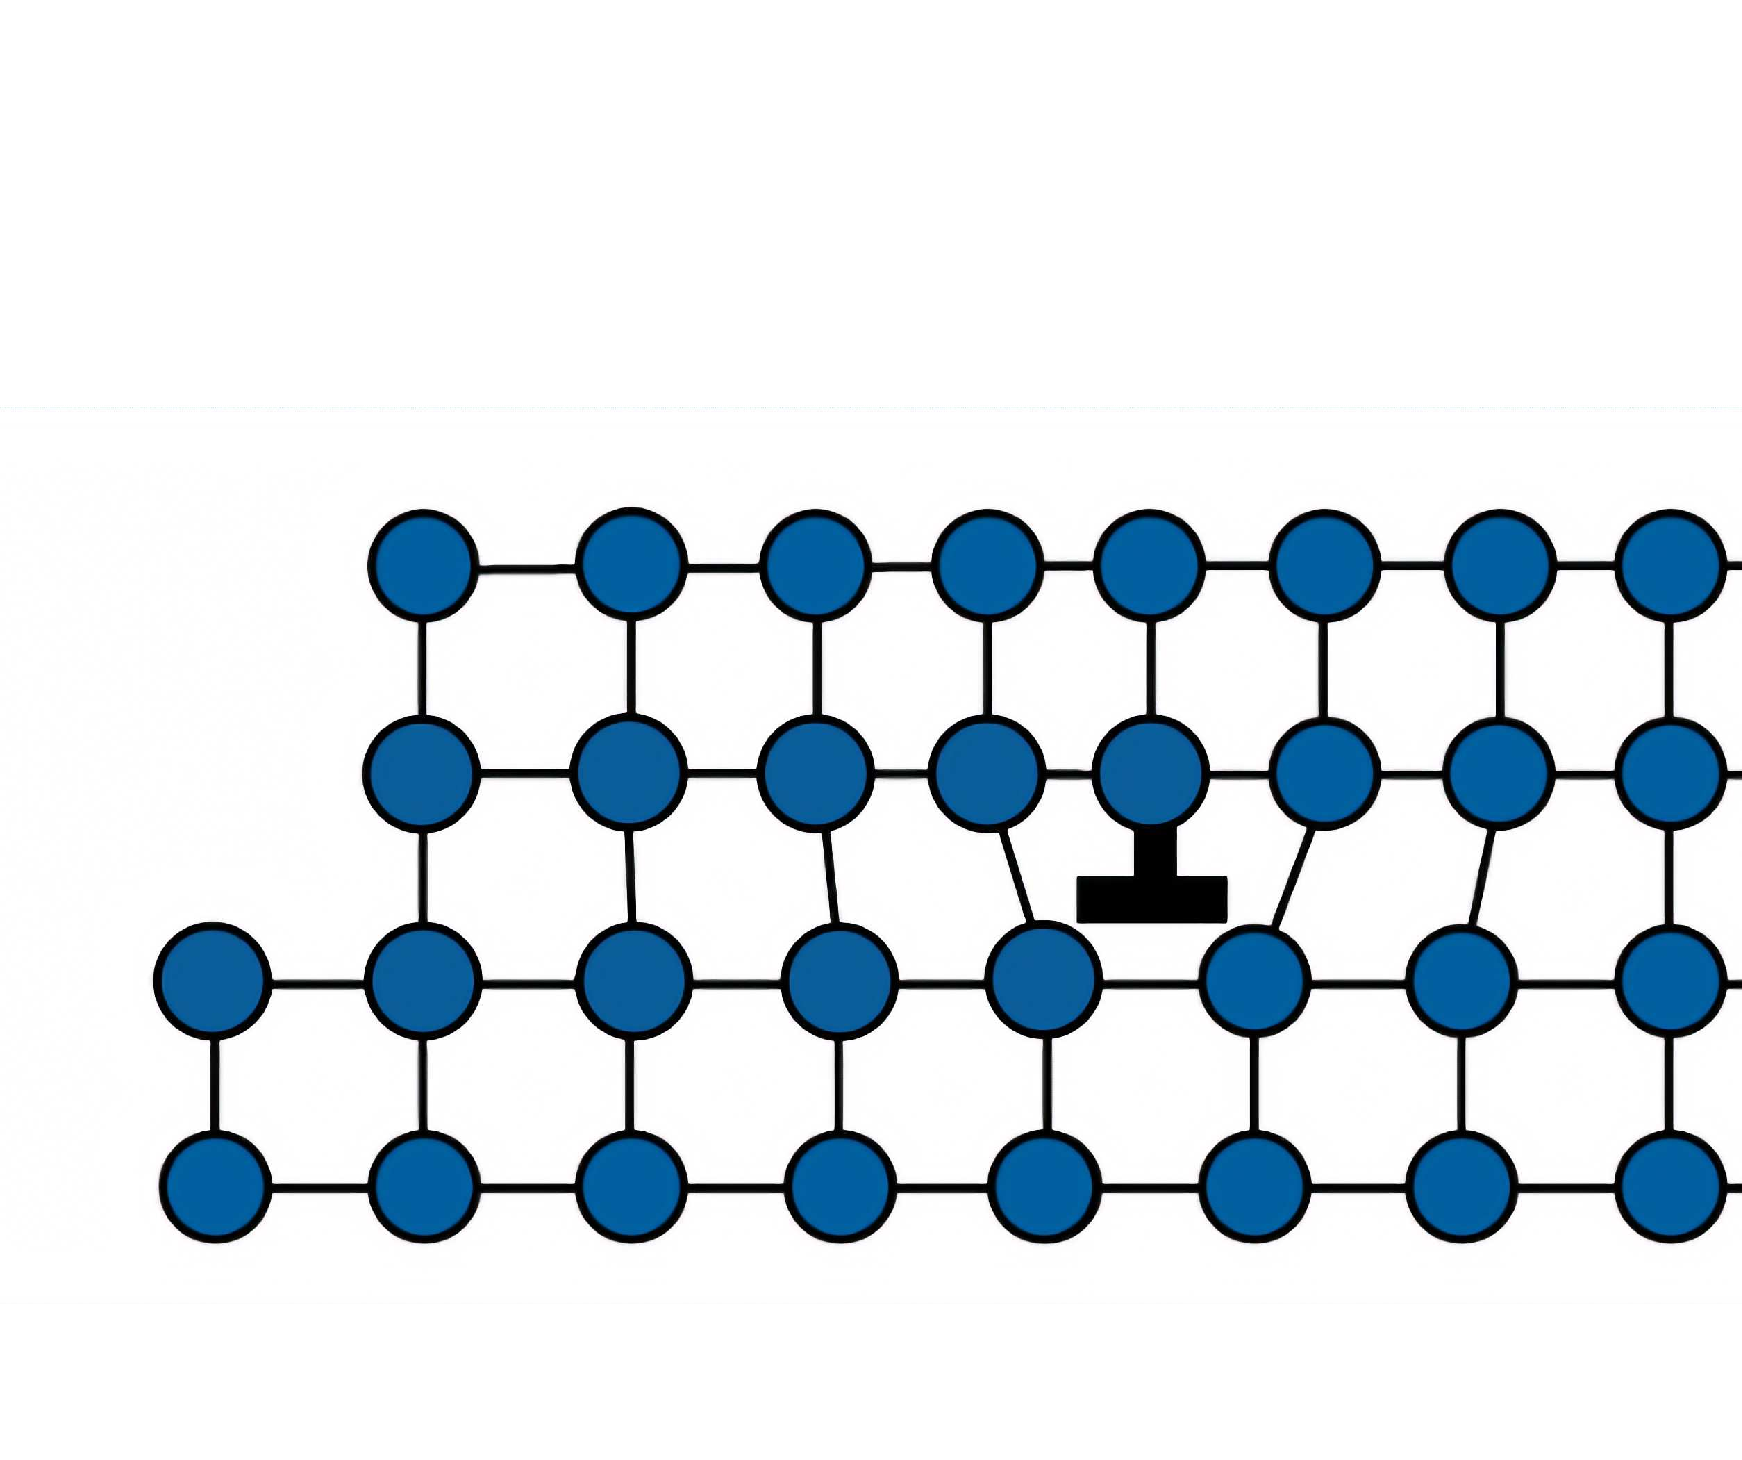
\includegraphics[width=0.9\linewidth, height=2.8cm, keepaspectratio]{figures_dr/fig_plasticity.pdf}

    \column{0.31\textwidth}
    \centering
    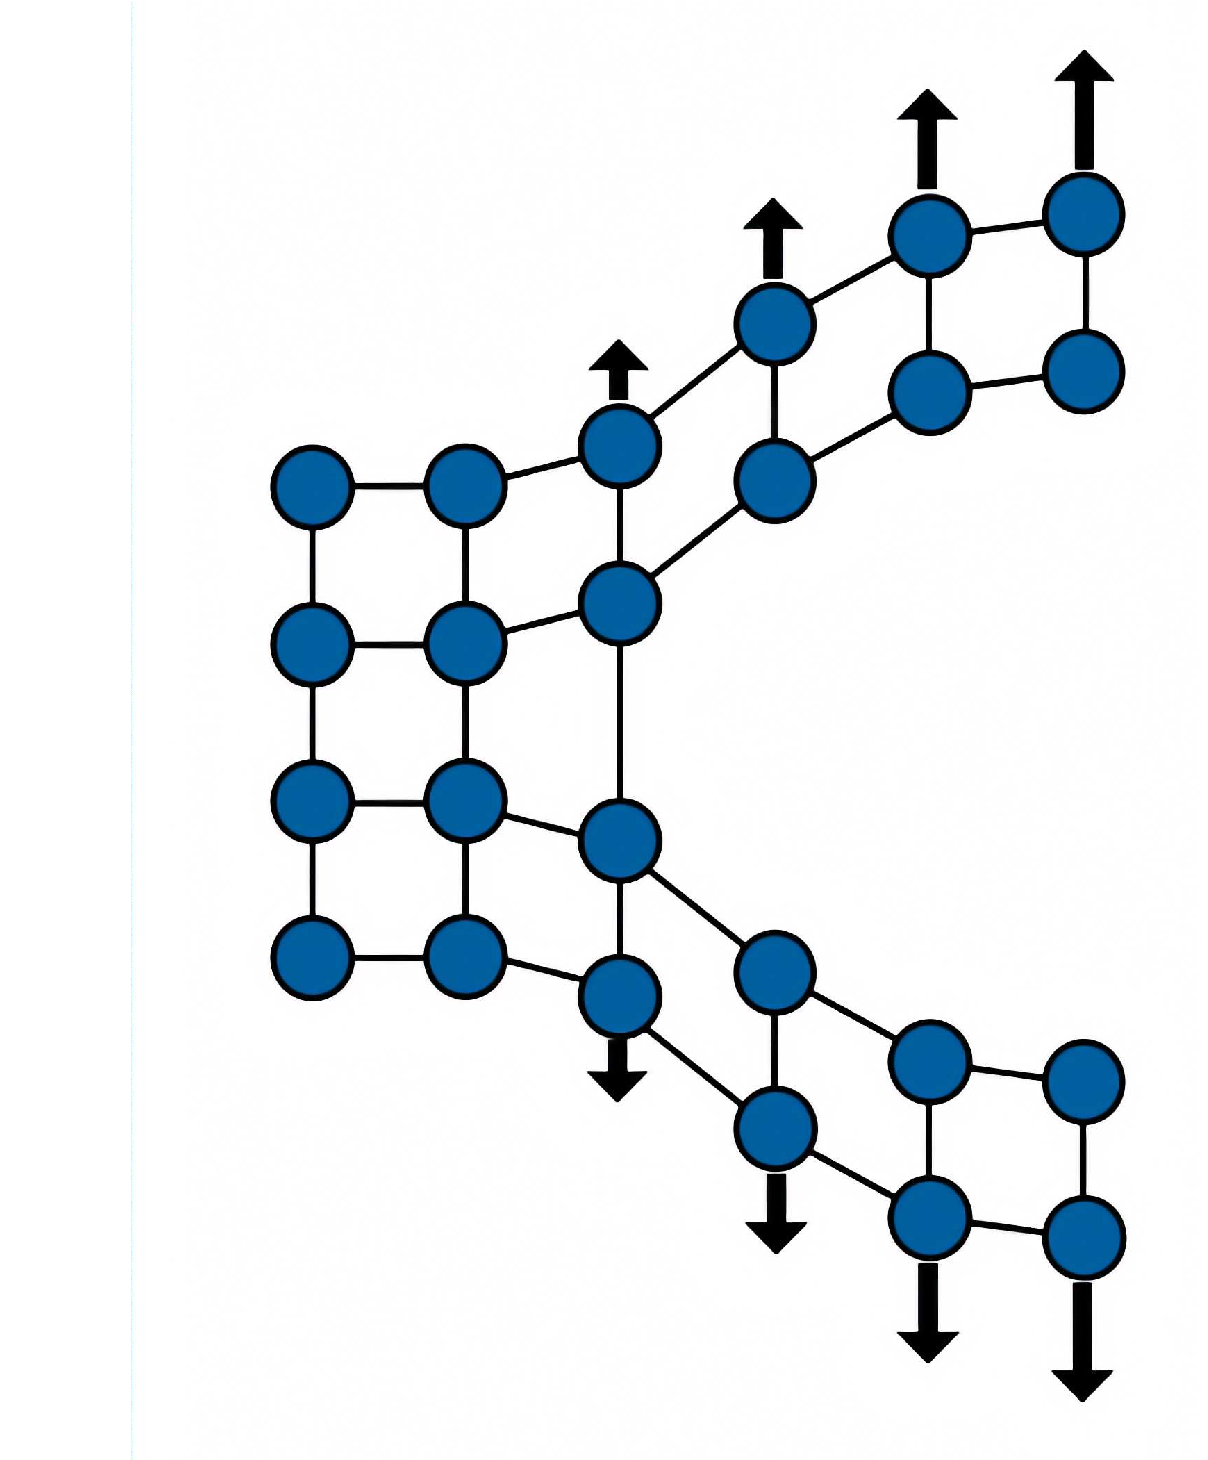
\includegraphics[width=0.9\linewidth, height=2.8cm, keepaspectratio]{figures_dr/fig_fracture.pdf}
\end{columns}

\vfill

% --- Methods footer ---
\textcolor{AcademicNavy!25}{\rule{\linewidth}{0.3pt}}
\vspace{0.03cm}
\begin{center}
{\scriptsize \color{AcademicNavy!80}
\textbf{Methods:}\enspace
Ginzburg-Landau Theory\enspace$\cdot$\enspace Phase-Field\enspace$\cdot$\enspace FEM\enspace$\cdot$\enspace Non-linear Elasticity
}
\end{center}

\vspace{0.15cm}

\end{frame}

% ===========================================================
% Slide 4: Phase Transitions
% ===========================================================
\begin{frame}{Phase Transitions}
\vspace*{-0.cm}

% ---- TOP: subtitles side by side ----
\begin{columns}[T, totalwidth=\textwidth]
    \column{0.48\textwidth}
    \textcolor{SteelBlue}{\rule{\linewidth}{0.8pt}}\\[0.06cm]
    {\small \textcolor{AcademicNavy}{\textbf{Martensitic — SMA}}}\\[0.03cm]
    {\scriptsize \textbf{Reversible} $|$ High sym. $\to$ Low sym.}

    \column{0.48\textwidth}
    \textcolor{SteelBlue}{\rule{\linewidth}{0.8pt}}\\[0.06cm]
    {\small \textcolor{AcademicNavy}{\textbf{Reconstructive — Ti, Zr}}}\\[0.03cm]
    {\scriptsize \textbf{Irreversible} $|$ High sym. $\to$ High sym.\enspace e.g. BCC $\to$ HCP}
\end{columns}

\vfill

% ---- 3 images aligned ----
\begin{columns}[c, totalwidth=\textwidth]
    \column{0.36\textwidth}
    \centering
    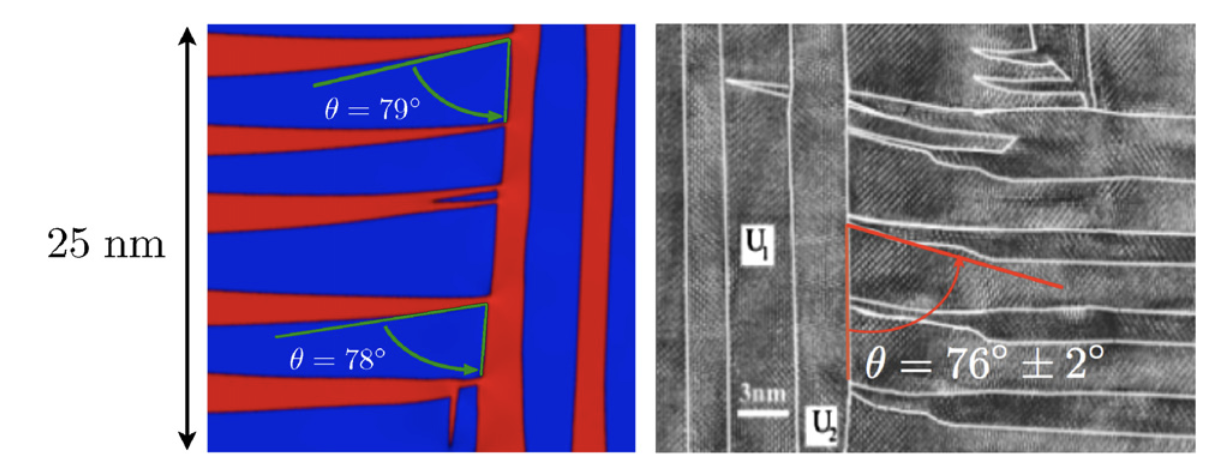
\includegraphics[width=\linewidth, height=1.8cm, keepaspectratio]{figures_dr/figsma.png}

    \column{0.30\textwidth}
    \centering
    {\tiny \color{AcademicNavy} BCC$\to$HCP}\\[0.03cm]
    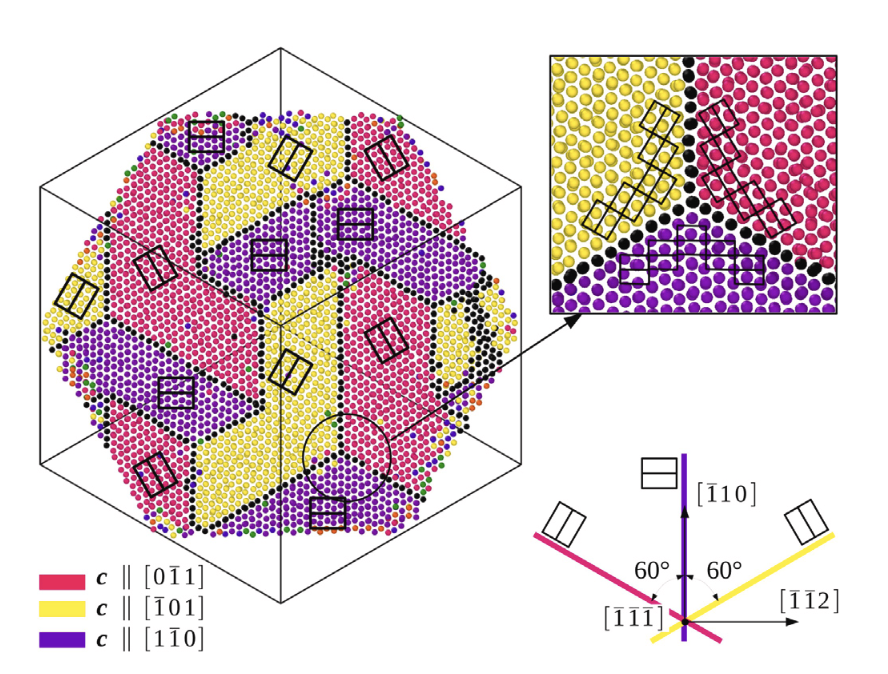
\includegraphics[width=\linewidth, height=1.8cm, keepaspectratio]{figures_dr/BCCHCP.png}

    \column{0.30\textwidth}
    \centering
    {\tiny \color{AcademicNavy} Square$\to$Triangular}\\[0.03cm]
    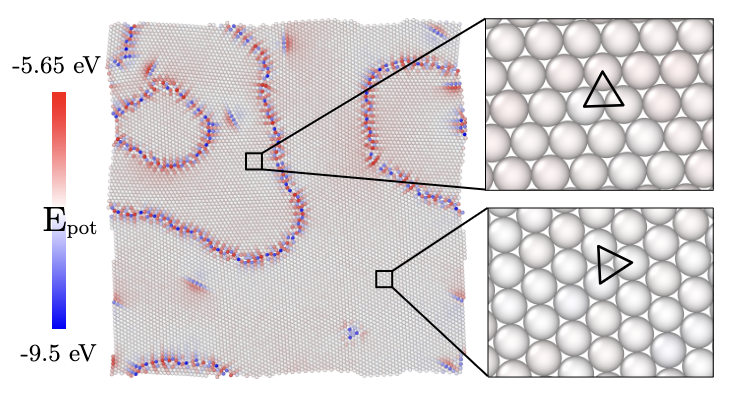
\includegraphics[width=\linewidth, height=1.8cm, keepaspectratio]{figures_dr/squretriangular.png}
\end{columns}

\vspace{0.03cm}
% ---- BOTTOM: discovery + refs spanning full width ----
\textcolor{AcademicNavy!25}{\rule{\linewidth}{0.3pt}}
\vspace{0.03cm}

{\scriptsize \color{SteelBlue}\textbf{Key discoveries:}}\\[0.03cm]
{\scriptsize
\begin{itemize}\setlength\itemsep{0.02cm}
    \item \textbf{Large elastic deformation framework} is necessary to describe solid-to-solid transitions
    \item In reconstructive transitions: \textbf{plastic slip} is the essential transformation carrier — not microscopic shuffling
    \item Transition proceeds via \textbf{lattice-invariant shears} between high-symmetry phases
    \item Development of a new \textbf{mesoscopic Landau theory} for reconstructive phase transitions
\end{itemize}
}
{\fontsize{5}{6}\selectfont \color{AcademicNavy!80}
    \textbf{PhD:}\enspace C. Baruffi\enspace|\enspace
    \textbf{Post-doc:}\enspace K. Ghosh\enspace|\enspace
    \textbf{Funding:}\enspace ONERA $\cdot$ ANR JCJC ALIS\enspace|\enspace
    \textbf{Pub:}\enspace Salman et al., \textit{C. R. Physique} (2019)\enspace$\cdot$\enspace
    Salman et al., \textit{Eur. J. Phys.} (2019)\enspace$\cdot$\enspace
    Baruffi et al., \textit{Comput. Mater. Sci.} (2022)\enspace$\cdot$\enspace
    Ghosh et al., \textit{Phys. Rev. Mater.} (2025)
}

\vfill
% --- Methods footer ---
\textcolor{AcademicNavy!25}{\rule{\linewidth}{0.3pt}}
%\vspace{0.03cm}
\begin{center}
{\scriptsize \color{AcademicNavy!80}
\textbf{Methods:}\enspace
Ginzburg-Landau Theory\enspace$\cdot$\enspace Phase-Field\enspace$\cdot$\enspace FEM\enspace$\cdot$\enspace Non-linear Elasticity
}
\end{center}

\end{frame}

% ===========================================================
% Slide 5: Macroscopic Response
% ===========================================================
% Slide 5: Wild-to-Mild Plasticity
% ===========================================================
\begin{frame}{Plasticity}
\vspace*{-0.2cm}

% ---- Header ----
\textcolor{SteelBlue}{\rule{\linewidth}{0.8pt}}\\[0.04cm]
{\small \textcolor{AcademicNavy}{\textbf{Wild-to-Mild Plasticity}} \hfill
{\scriptsize \textbf{Size \& disorder effects} in crystal plasticity — Pure Al, Al-Sc, Al-Sc precipitate, Al-Cu-Sn}}

\vfill

% ---- TOP ROW: two images side by side ----
\begin{columns}[c, totalwidth=\textwidth]
    \column{0.50\textwidth}
    \centering
    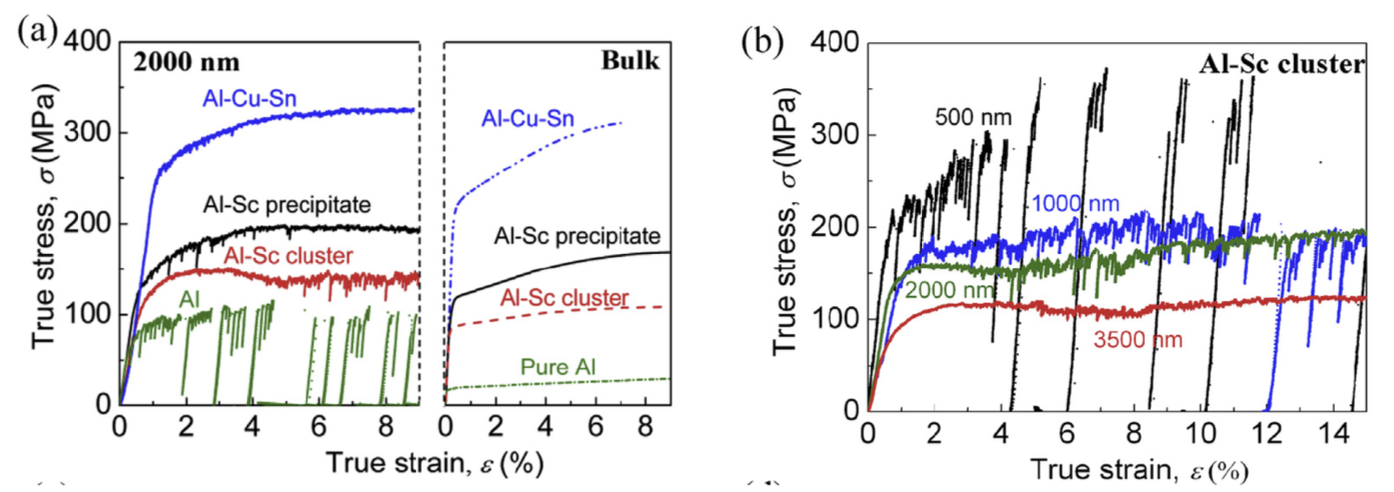
\includegraphics[width=\linewidth, height=1.85cm, keepaspectratio]{figures_dr/s5-2.png}

    \column{0.48\textwidth}
    \centering
    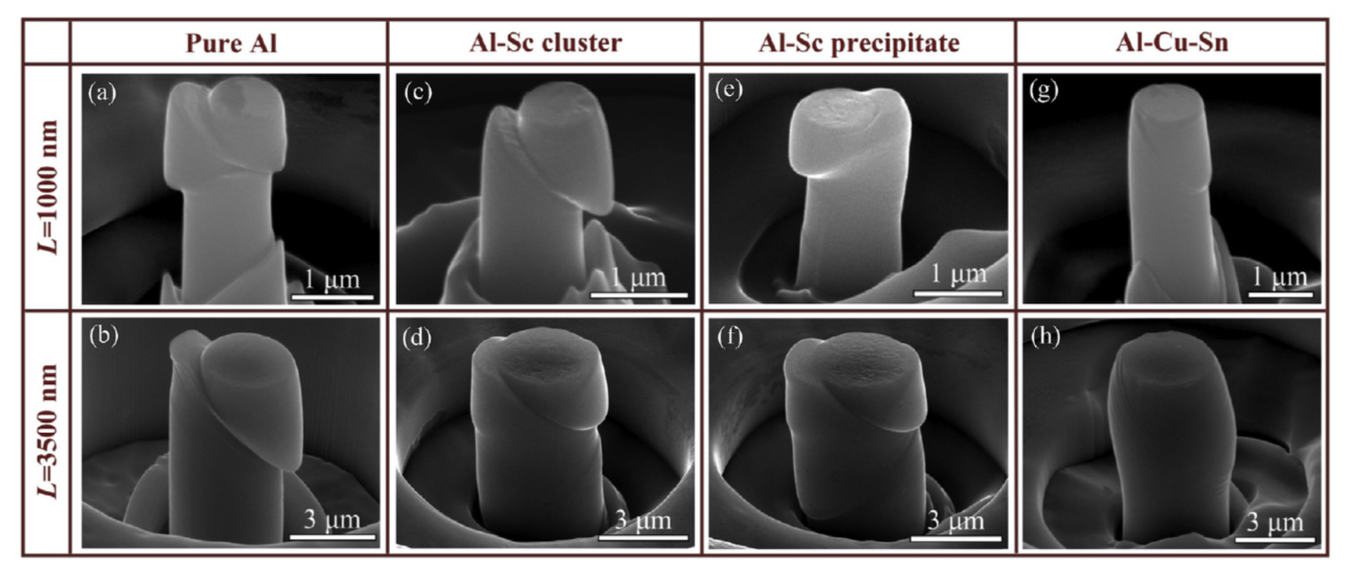
\includegraphics[width=\linewidth, height=1.85cm, keepaspectratio]{figures_dr/s5-1.png}
\end{columns}

\vspace{0.2cm}
% ---- BOTTOM: key discoveries + refs ----
\textcolor{AcademicNavy!25}{\rule{\linewidth}{0.3pt}}

{\scriptsize \color{SteelBlue}\textbf{Key discoveries:}}\\[0.01cm]
{\scriptsize
\begin{itemize}\setlength\itemsep{0.1cm}
    \item \textbf{Disorder \& size} suppress intermittent ``wild'' $\to$ smooth ``mild'' flow
    \item Avalanches follow \textbf{scale-free statistics} — signature of criticality
    \item \textbf{Disorder is tailorable} to drive a brittle-to-ductile transition
    \item \textbf{Automaton model:} three-stage crossover — spin-glass (small/pure) $\to$ spinodal/depinning (intermediate) $\to$ brittle-ductile (large/disordered)
\end{itemize}
}
{\fontsize{5}{6}\selectfont \color{AcademicNavy!80}
    \textbf{PhD:}\enspace P. Zhang\enspace|\enspace
    \textbf{Funding:}\enspace ANR SUMMIT\enspace|\enspace
    \textbf{Pub:}\enspace Salman et al., \textit{PRL} (2011)\enspace$\cdot$\enspace
    Zhang et al., \textit{Acta Mater.} (2017)\enspace$\cdot$\enspace
    Zhang et al., \textit{PRE} (2020)\enspace$\cdot$\enspace
    Weiss et al., \textit{C. R. Physique} (2021)
}
\vfill
% --- Methods footer ---
\textcolor{AcademicNavy!25}{\rule{\linewidth}{0.3pt}}
%\vspace{1cm}
\begin{center}
{\scriptsize \color{AcademicNavy!80}
\textbf{Methods:}\enspace
Ginzburg-Landau Theory\enspace$\cdot$\enspace Phase-Field\enspace$\cdot$\enspace FEM\enspace$\cdot$\enspace Non-linear Elasticity
}
\end{center}

\end{frame}

% ===========================================================
% Slide 6: Plasticity — Formalism & Large Deformation
% ===========================================================
\begin{frame}{Plasticity}
\vspace*{-0.2cm}

% ---- Row 1 ----
\textcolor{SteelBlue}{\rule{\linewidth}{0.8pt}}\\[0.03cm]
{\small \textcolor{AcademicNavy}{\textbf{Time-discontinuous elasto-plasticity formalism}}}

\vspace{0.08cm}

\begin{columns}[c, totalwidth=\textwidth]
    \column{0.38\textwidth}
    \centering
    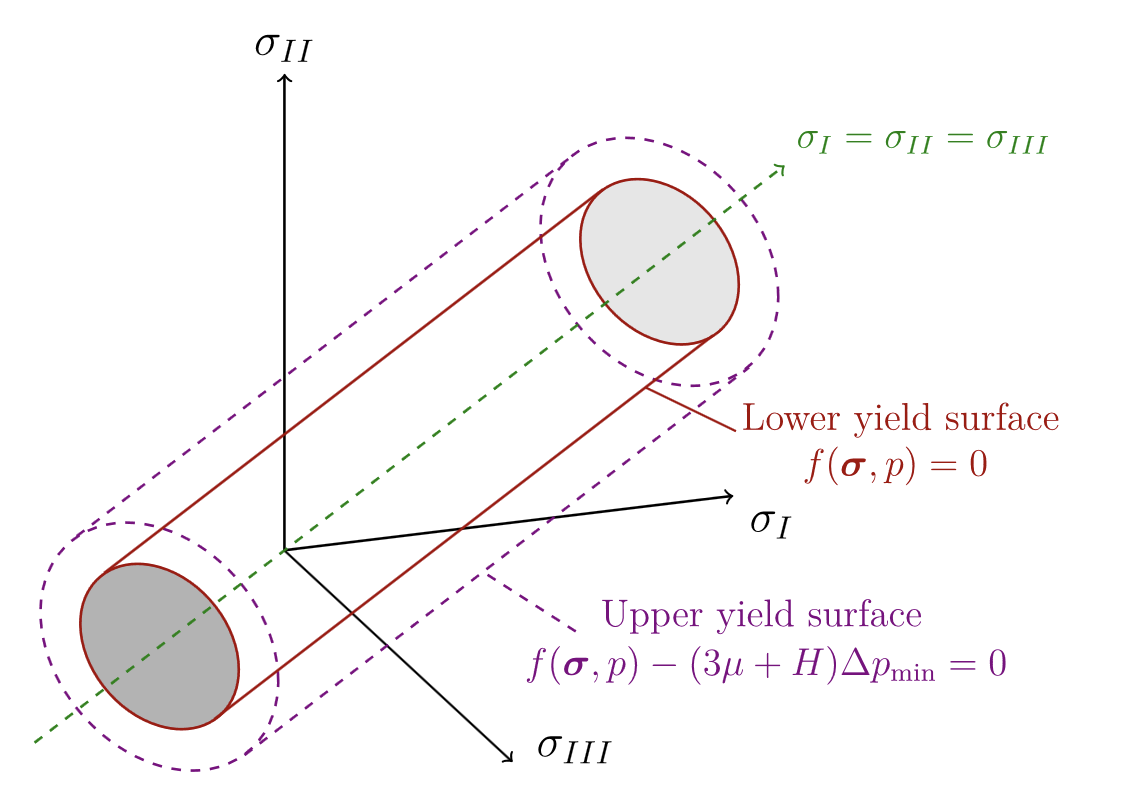
\includegraphics[width=\linewidth, height=2.5cm, keepaspectratio]{figures_dr/s6-1.png}

    \column{0.58\textwidth}
    \centering
    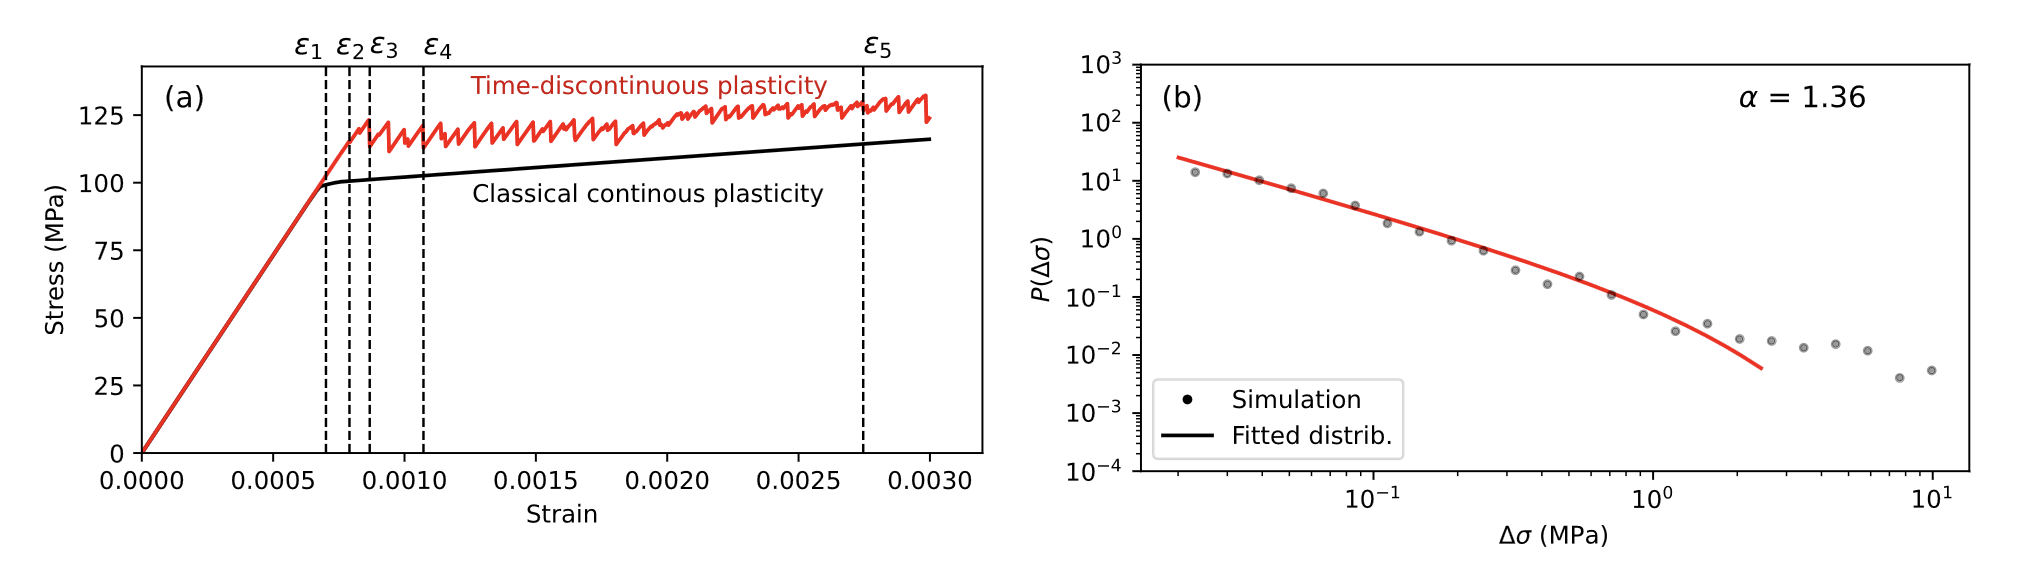
\includegraphics[width=\linewidth, height=3.0cm, keepaspectratio]{figures_dr/s6-2.png}
\end{columns}

\vspace{0.03cm}
{\fontsize{5}{6}\selectfont \color{AcademicNavy!80}
    \textbf{Post-doc:}\enspace M. Lamari\enspace|\enspace
    \textbf{Funding:}\enspace ANR Mesocrysp\enspace|\enspace
    \textbf{Pub:}\enspace Lamari et al., \textit{Int. J. Solids Struct.} (2024)
}

\vspace{0.1cm}

% ---- Row 2 ----
\textcolor{SteelBlue}{\rule{\linewidth}{0.8pt}}\\[0.03cm]
{\small \textcolor{AcademicNavy}{\textbf{Large deformation Arbitrary Lagrangian–Eulerian plasticity}}}

\vspace{0.08cm}

\begin{columns}[c, totalwidth=\textwidth]
    \column{0.48\textwidth}
    \centering
    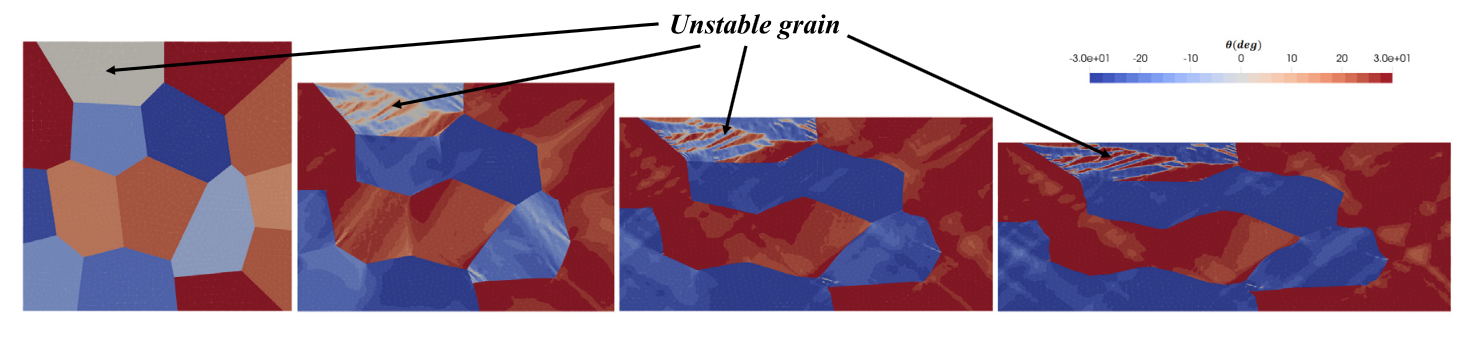
\includegraphics[width=\linewidth, height=2.2cm, keepaspectratio]{figures_dr/s6-3.png}

    \column{0.48\textwidth}
    \centering
    \raisebox{0.35cm}{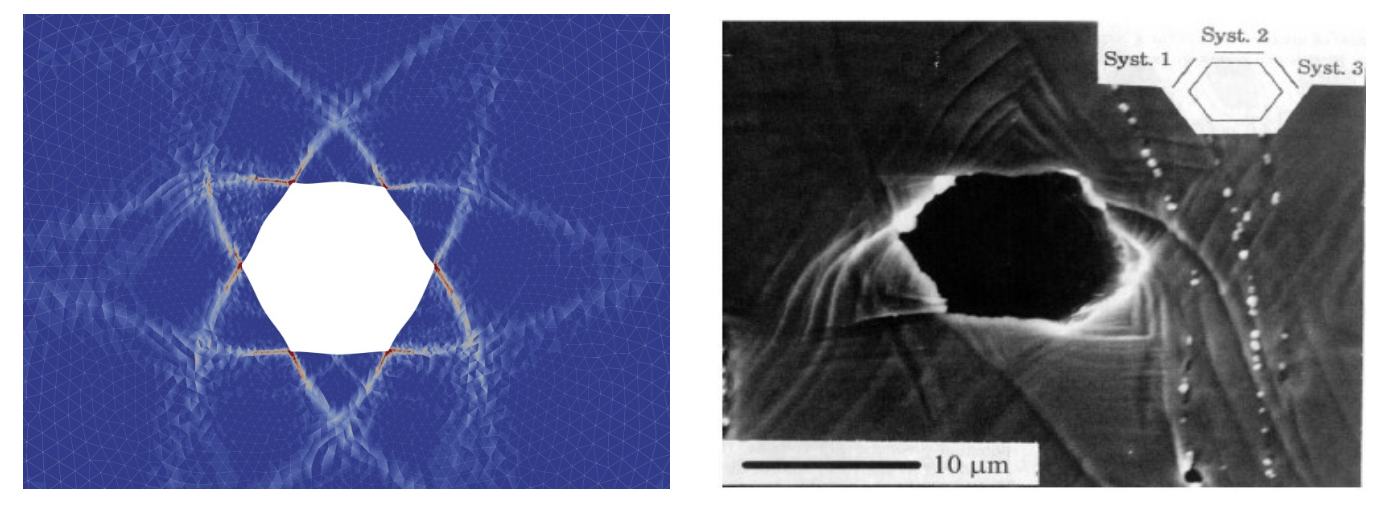
\includegraphics[width=\linewidth, height=2.2cm, keepaspectratio]{figures_dr/s6-4.png}}
\end{columns}

\vspace{0.03cm}
{\fontsize{5}{6}\selectfont \color{AcademicNavy!80}
    \textbf{PhD:}\enspace J. Smiri\enspace|\enspace
    \textbf{Funding:}\enspace Bourse Ministère, Coup de pouce F2M \enspace|\enspace
    \textbf{Pub:}\enspace Smiri et al., \textit{Eur. J. Mech.-A/Solids} (2023)\enspace$\cdot$\enspace
    Smiri et al., \textit{Int. J. Solids Struct.} (2024)
}
\vfill
% --- Methods footer ---
\textcolor{AcademicNavy!25}{\rule{\linewidth}{0.3pt}}
%\vspace{0.03cm}
\begin{center}
{\scriptsize \color{AcademicNavy!80}
\textbf{Methods:}\enspace
Ginzburg-Landau Theory\enspace$\cdot$\enspace Phase-Field\enspace$\cdot$\enspace FEM\enspace$\cdot$\enspace Non-linear Elasticity
}
\end{center}

\end{frame}

% ===========================================================
% Slide 7: Lattice Symmetry & Metric Space
% ===========================================================
\begin{frame}{Lattice Symmetry \& Metric Space}
\vspace*{-0.2cm}

% ---- Row 1: Lattice symmetry ----
\textcolor{SteelBlue}{\rule{\linewidth}{0.8pt}}\\[0.03cm]
{\small \textcolor{AcademicNavy}{\textbf{Lattice symmetry}}}

\vspace{0.08cm}

\begin{columns}[c, totalwidth=\textwidth]
    \column{0.55\textwidth}
    {\scriptsize
    \begin{tabular}{p{2.1cm} l}
        \textbf{\color{SecondaryTitle} Bravais lattice:} & $\mathcal{L}(\mathbf{e}_I) = \{ v_I \mathbf{e}_I,\ v_I \in \mathbb{Z} \}$ \\[0.18cm]
        \textbf{\color{SecondaryTitle} Lattice metric:} & $C_{IJ} = \mathbf{e}_I \cdot \mathbf{e}_J$ \\[0.18cm]
        \textbf{\color{SecondaryTitle} Non-uniqueness:} & $\bar{\mathbf{e}}_J = M_{IJ} \mathbf{e}_I,\ \mathbf{M} \in GL(2,\mathbb{Z})$ \\[0.18cm]
        \textbf{\color{SecondaryTitle} $GL(2,\mathbb{Z})$:} & $\{ \mathbf{M},\ \det(\mathbf{M}) = \pm 1 \}$ \\[0.18cm]
        \textbf{\color{SecondaryTitle} Metric transform:} & $\bar{\mathbf{C}} = \mathbf{M}^T \mathbf{C} \mathbf{M}$ \\[0.18cm]
        \textbf{\color{SecondaryTitle} $\mathbf{C} = \mathbf{F}^T\mathbf{F}$:} & $C_{IJ} = \mathbf{e}_I\cdot(\mathbf{F}^T\mathbf{F})\mathbf{e}_J$
    \end{tabular}
    }

    \column{0.42\textwidth}
    \centering
    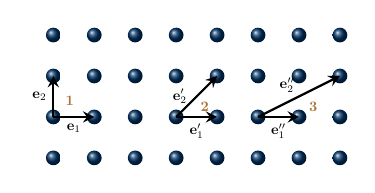
\begin{tikzpicture}[>=stealth, scale=0.52, every node/.style={transform shape}]
        \foreach \x in {0,...,7} {
            \foreach \y in {0,...,3} {
                \shade[ball color=AcademicNavy] (\x,\y) circle (0.18);
            }
        }
        \draw[->, thick] (0,1) -- (1,1) node[midway, below=1pt] {$\mathbf{e}_1$};
        \draw[->, thick] (0,1) -- (0,2) node[midway, left=1pt] {$\mathbf{e}_2$};
        \node[text=brown!90!black, font=\bfseries] at (0.4, 1.4) {1};
        \draw[->, thick] (3,1) -- (4,1) node[midway, below=1pt] {$\mathbf{e}_1'$};
        \draw[->, thick] (3,1) -- (4,2) node[midway, left=3pt] {$\mathbf{e}_2'$};
        \node[text=brown!90!black, font=\bfseries] at (3.7, 1.25) {2};
        \draw[->, thick] (5,1) -- (6,1) node[midway, below=1pt] {$\mathbf{e}_1''$};
        \draw[->, thick] (5,1) -- (7,2) node[midway, above left=-1pt] {$\mathbf{e}_2''$};
        \node[text=brown!90!black, font=\bfseries] at (6.35, 1.25) {3};
    \end{tikzpicture}
\end{columns}

\vspace{0.3cm}

% ---- Row 2: Metric space ----
\textcolor{SteelBlue}{\rule{\linewidth}{0.8pt}}\\[0.03cm]
{\small \textcolor{AcademicNavy}{\textbf{Metric space: Poincaré projection \& lattice invariant shears}}\hfill{\scriptsize $\det\mathbf{C}=1$}}

\vspace{0.1cm}

\begin{columns}[c, totalwidth=\textwidth]
    \column{0.48\textwidth}
    \centering
    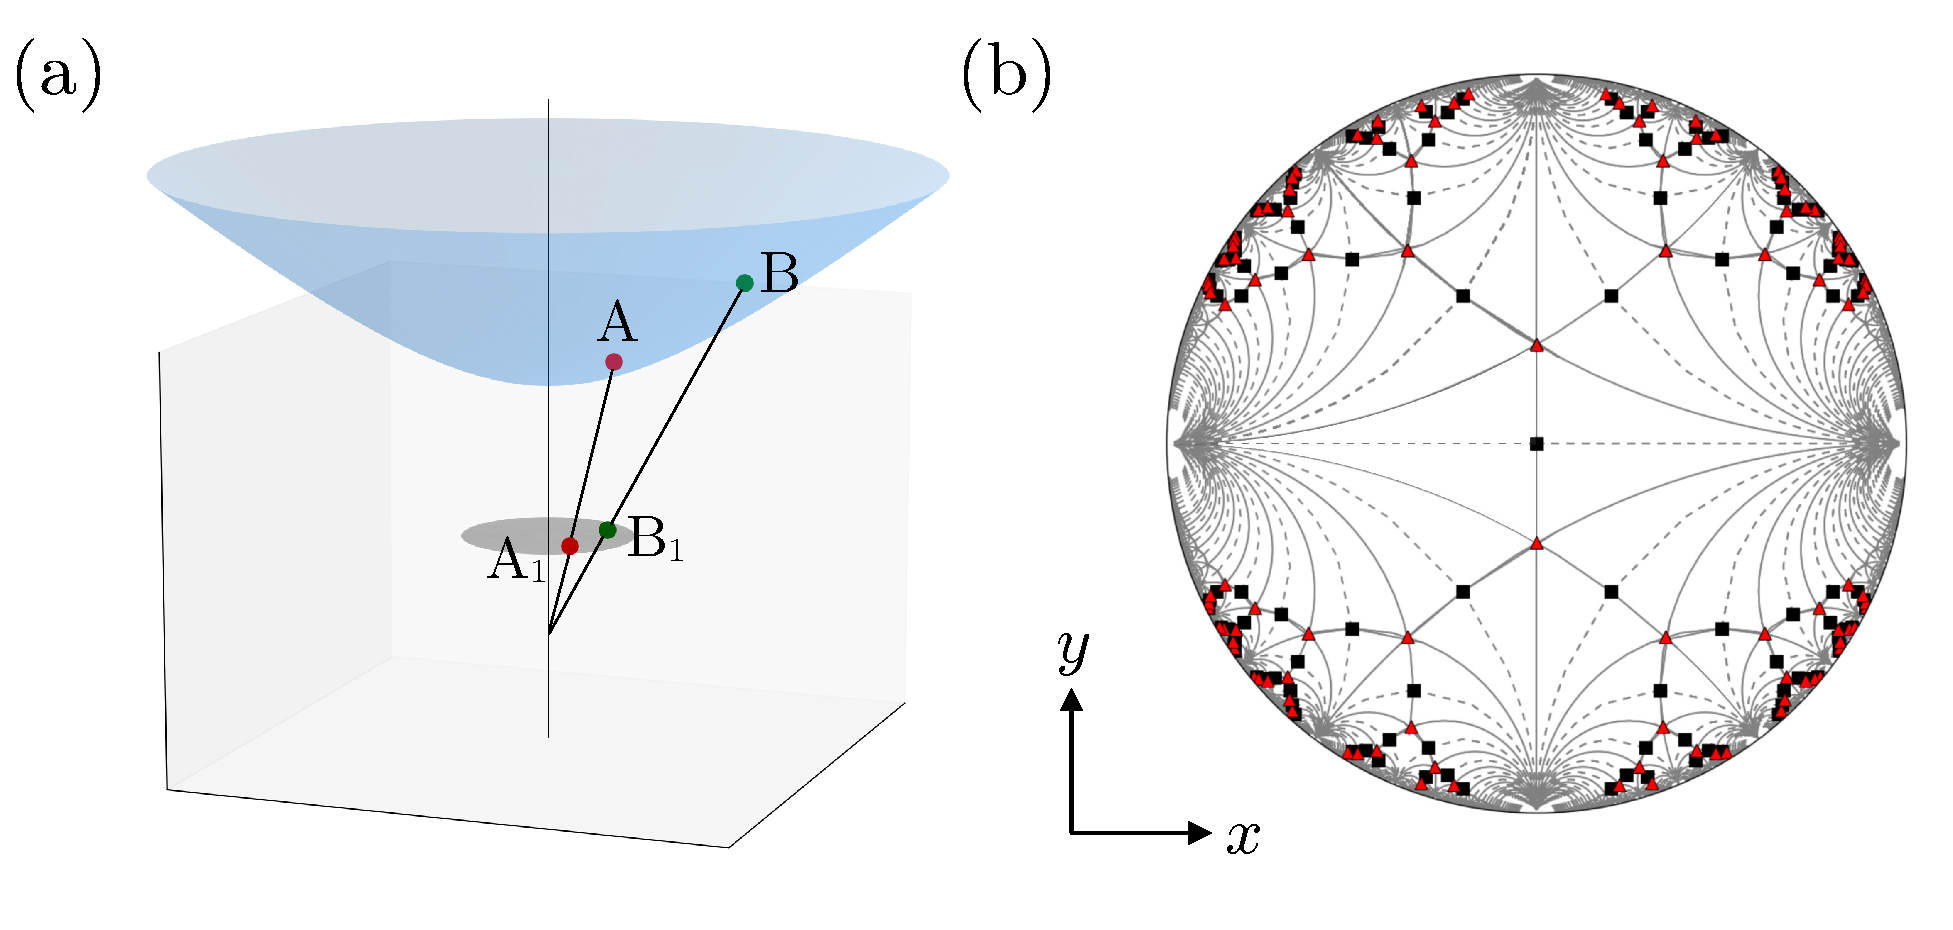
\includegraphics[width=\textwidth, height=4.2cm, keepaspectratio]{Figures/Figure2.pdf}

    \column{0.48\textwidth}
    \centering
    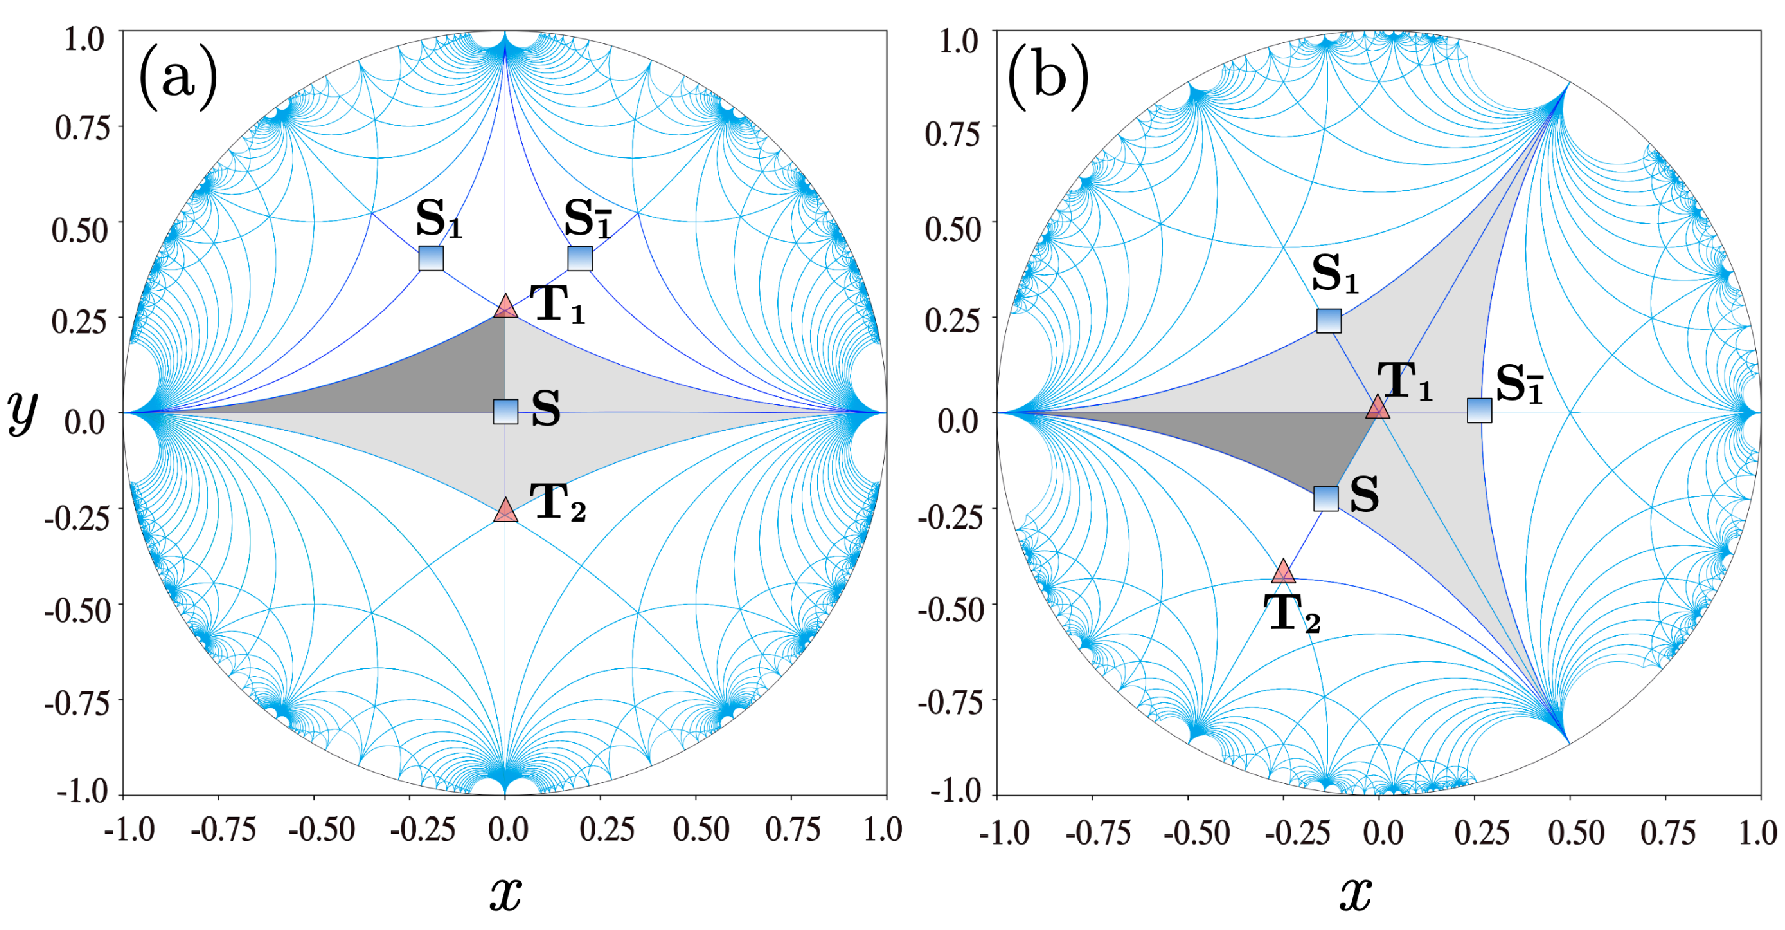
\includegraphics[width=\textwidth, height=4.2cm, keepaspectratio]{Figures/Figure3.pdf}
\end{columns}


\end{frame}

% ===========================================================
% Slide 8: Energy Landscape & Constructing Landau Energy
% ===========================================================
\begin{frame}{Energy Landscape \& Landau Energy Construction}
\vspace*{-0.2cm}

% ---- Images row ----
\begin{columns}[c, totalwidth=\textwidth]
    \column{0.38\textwidth}
    \centering
    {\scriptsize \color{AcademicNavy}\textbf{Energy landscape — square crystal}}\\[0.08cm]
    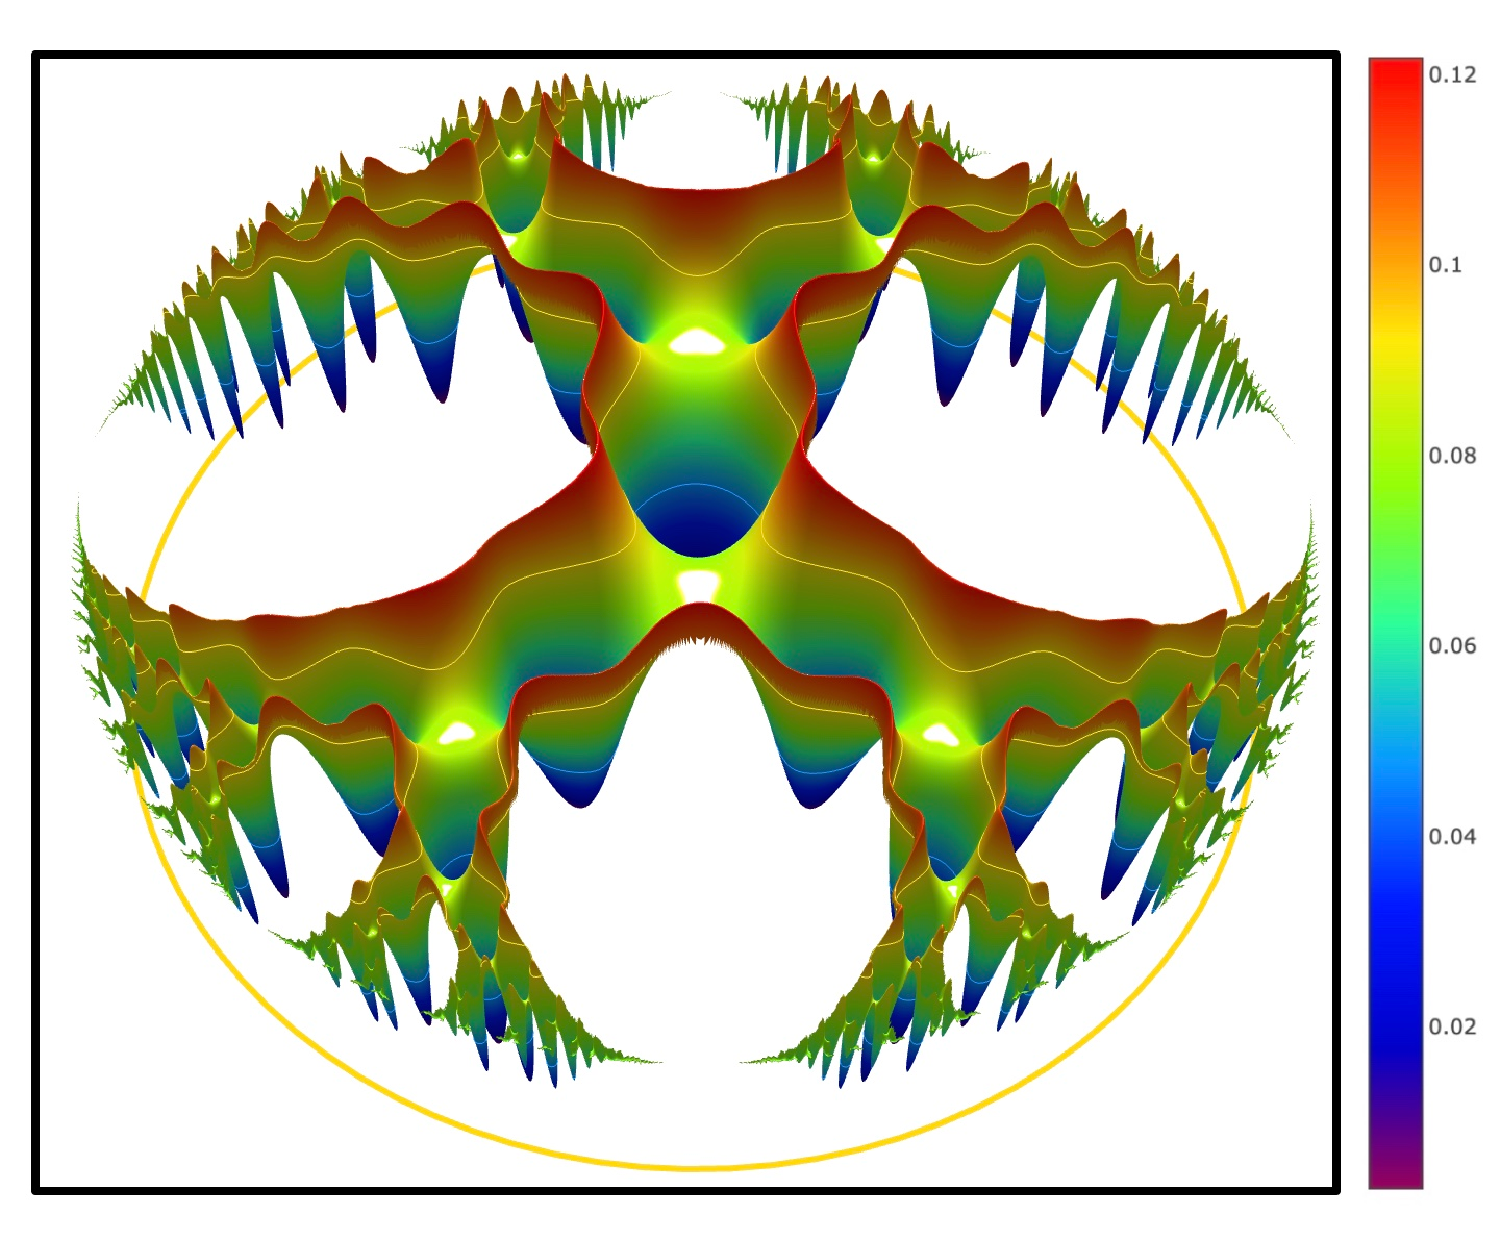
\includegraphics[width=\textwidth, height=3.2cm, keepaspectratio]{Figures/Fig1-b.pdf}

    \column{0.58\textwidth}
    \centering
    {\scriptsize \color{AcademicNavy}\textbf{Constructing the Landau energy}}\\[0.08cm]
    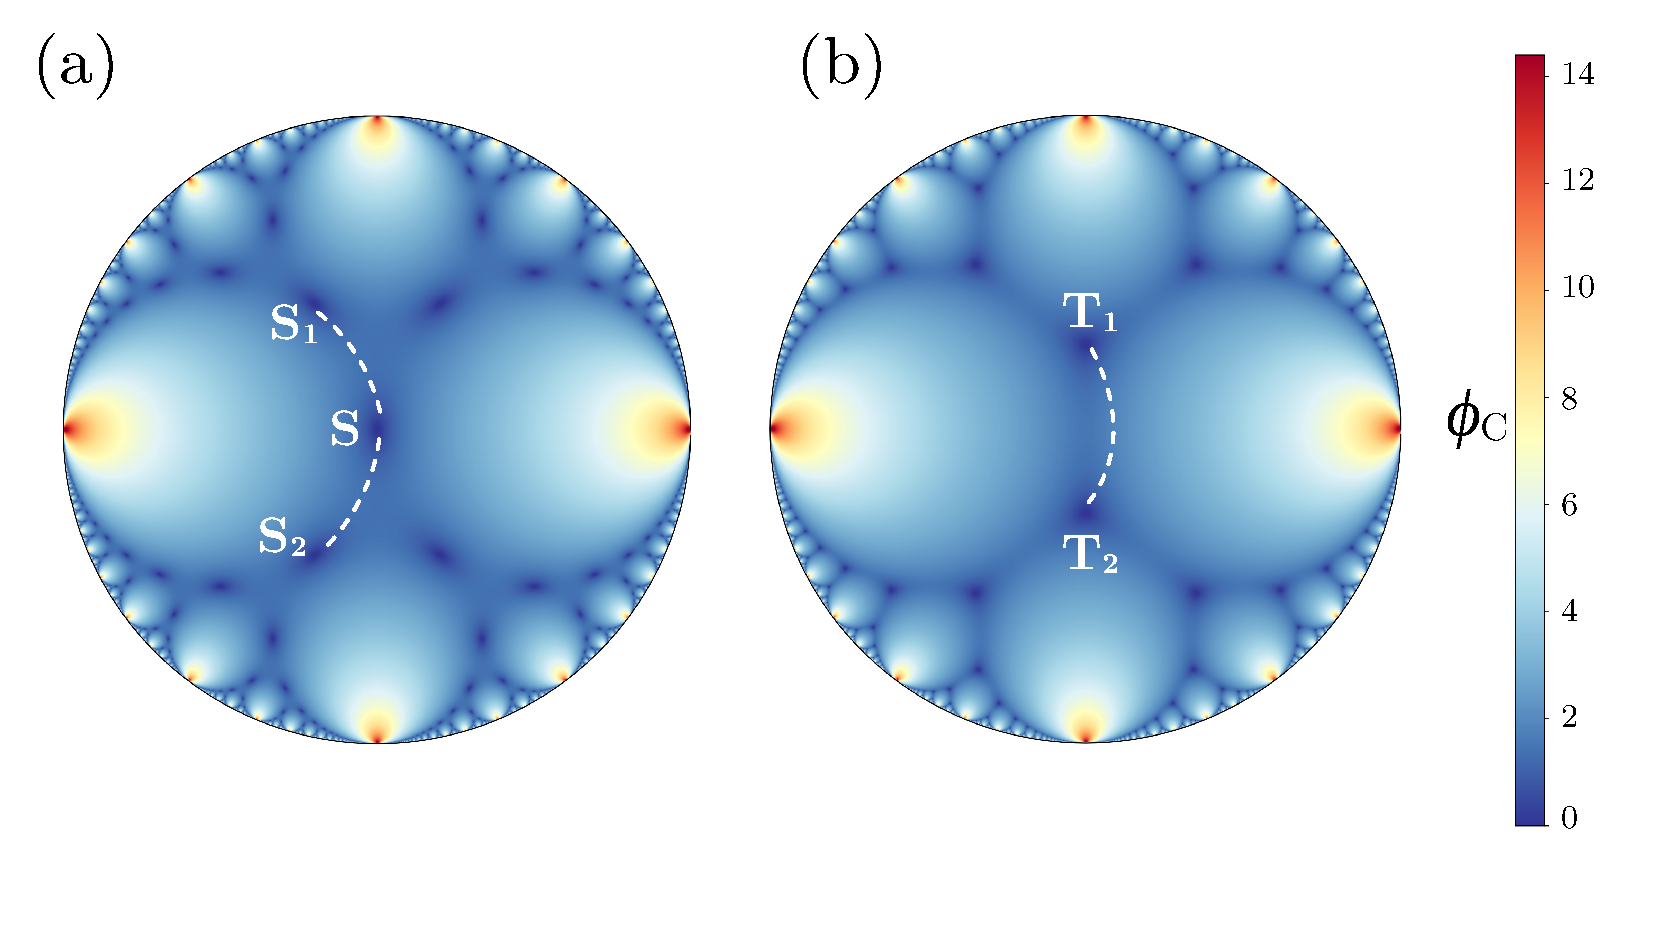
\includegraphics[width=\textwidth, height=3.2cm, keepaspectratio]{Figures/Figure5.pdf}
\end{columns}

\vspace{0.2cm}

% ---- Text ----
\textcolor{AcademicNavy!25}{\rule{\linewidth}{0.3pt}}
\vspace{0.05cm}

{\scriptsize
\begin{itemize}\setlength\itemsep{0.1cm}
    \item[\color{SteelBlue}\faAngleRight] $W(\mathbf{C})$ has \textbf{multiple wells} — each well is a symmetry-related variant
    \item[\color{SteelBlue}\faAngleRight] \textbf{Cauchy-Born rule:} $W(\mathbf{C})$ inherited from atomistic potential via $\mathbf{C} = \mathbf{F}^T\mathbf{F}$
    \item[\color{SteelBlue}\faAngleRight] \textbf{Polynomial construction:} symmetry-adapted polynomials enforcing \textbf{continuity across domain walls}
\end{itemize}
}

\end{frame}

% ===========================================================
% Slide 9: Numerical Results — MTM microstructure evolution
% ===========================================================
\begin{frame}{Numerical Results}
\vspace*{-0.2cm}

% ---- Images row ----
\begin{columns}[c, totalwidth=\textwidth]
    \column{0.55\textwidth}
    \centering
    \animategraphics[autoplay,loop,width=\linewidth]{5}{fps_frames/frame_}{001}{243}

    \column{0.42\textwidth}
    \centering
    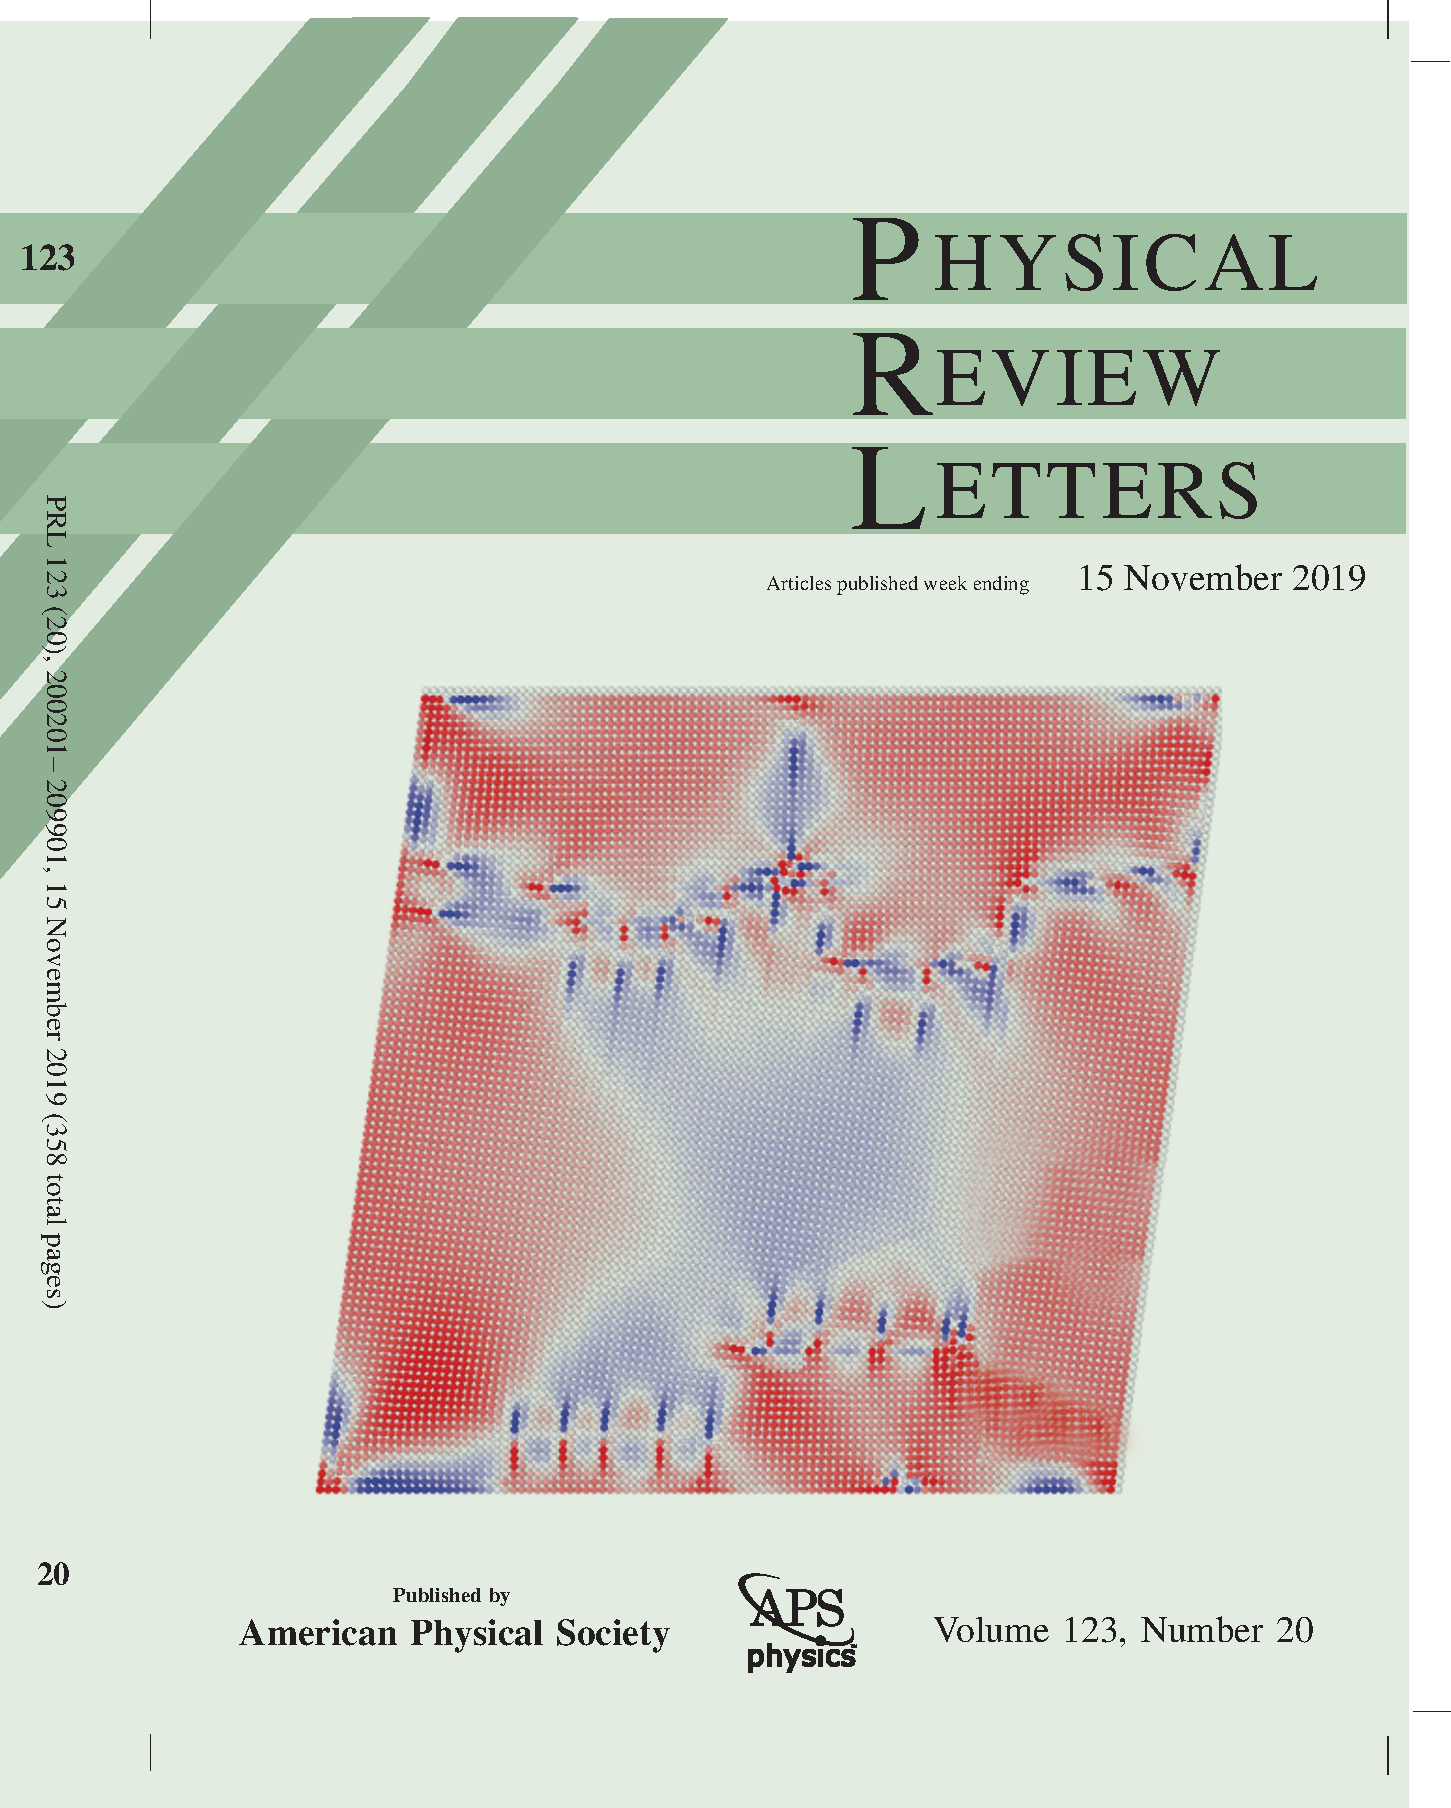
\includegraphics[width=0.78\linewidth, height=5.5cm, keepaspectratio]{Figures/LD16854cvr_copie.pdf}\\[0.05cm]
    {\fontsize{5}{6}\selectfont \color{AcademicNavy!70} Baggio et al., \textit{Phys. Rev. Lett.} (2019)}
\end{columns}

\vspace{0.1cm}
\textcolor{AcademicNavy!25}{\rule{\linewidth}{0.3pt}}
\vspace{0.03cm}

{\fontsize{5}{6}\selectfont \color{AcademicNavy!80}
    \textbf{PhD:}\enspace R. Baggio\enspace|\enspace
    \textbf{Funding:}\enspace ANR MesoCrysp\enspace|\enspace
    \textbf{Pub:}\enspace
    Baggio et al., \textit{PRL} (2019)\enspace$\cdot$\enspace
    Salman et al., \textit{C. R. Physique} (2021)\enspace$\cdot$\enspace
    Baggio et al., \textit{PRE} (2023)\enspace$\cdot$\enspace
    Baggio et al., \textit{Eur. J. Mech.} (2023)\enspace$\cdot$\enspace
    Salman et al., \textit{PRL} (2026)\enspace$\cdot$\enspace
}


\end{frame}

% ===========================================================
% Slide 10: Critical Exponents & Rebonding in Action
% ===========================================================
\begin{frame}{Critical Exponents \& Rebonding in Action}
\vspace*{-0.2cm}

% ---- Row 1: Critical exponents ----
\textcolor{SteelBlue}{\rule{\linewidth}{0.8pt}}\\[0.03cm]
{\small \textcolor{AcademicNavy}{\textbf{Critical exponents and finite-size scaling}}}

\vspace{0.08cm}

\begin{columns}[c, totalwidth=\textwidth]
    \column{0.44\textwidth}
    \centering
    \begin{tabular}{cc}
        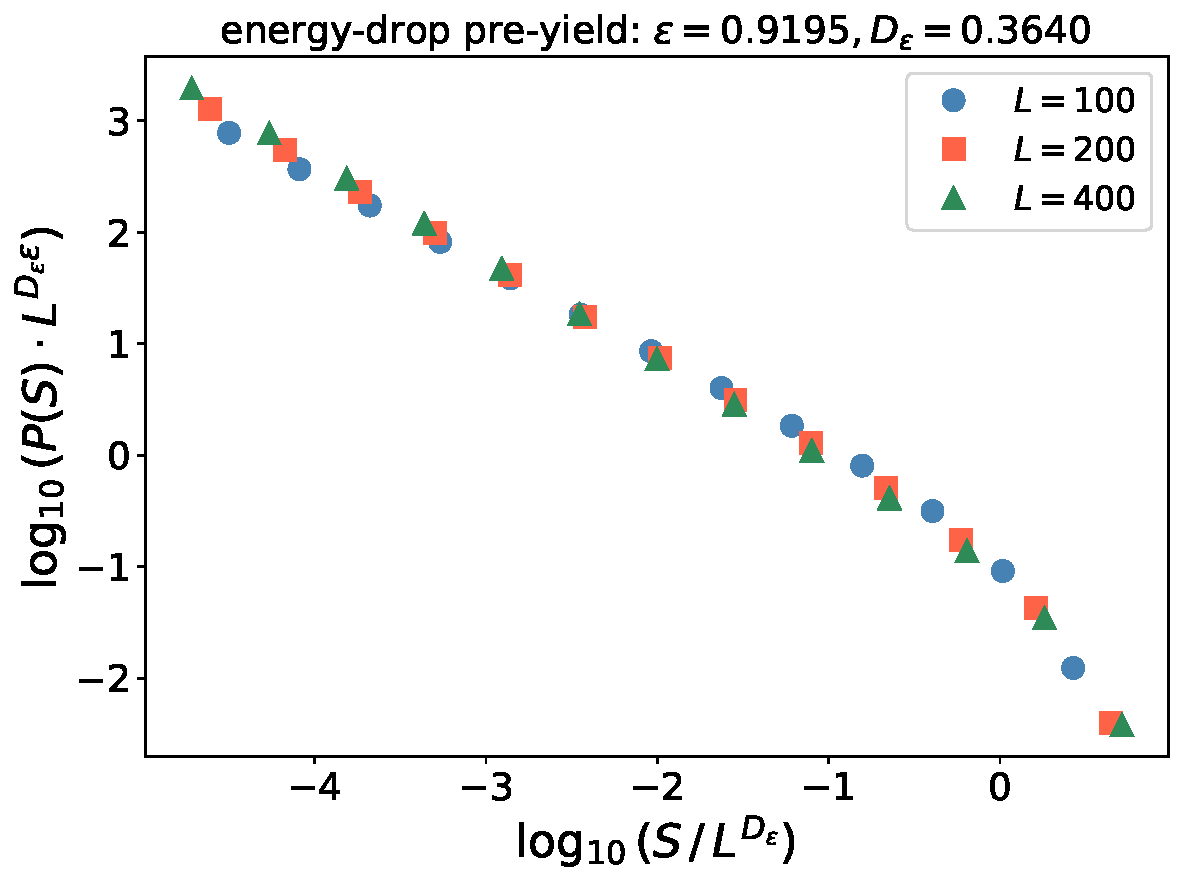
\includegraphics[width=0.48\linewidth]{Figures/Fig6-a.pdf} &
        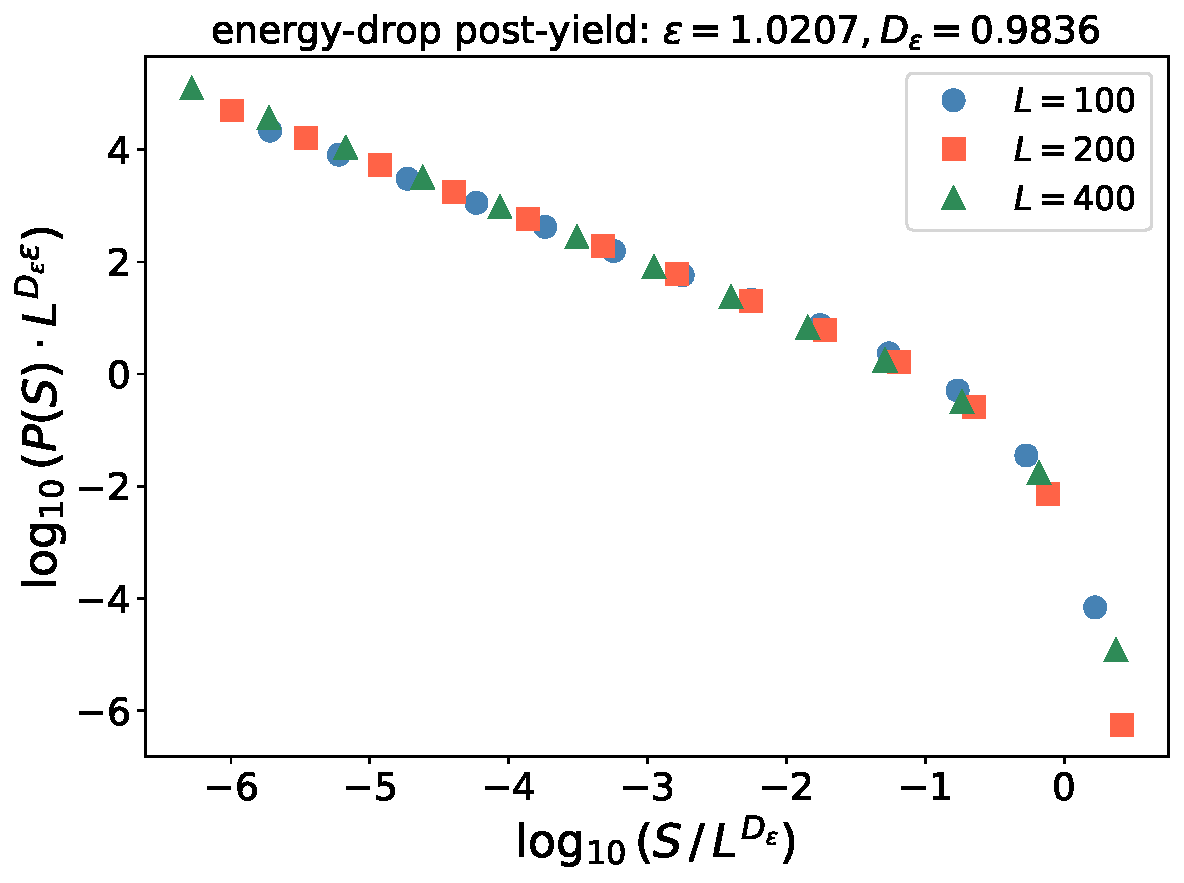
\includegraphics[width=0.48\linewidth]{Figures/Fig6-b.pdf}
    \end{tabular}

    \column{0.52\textwidth}
    \centering
    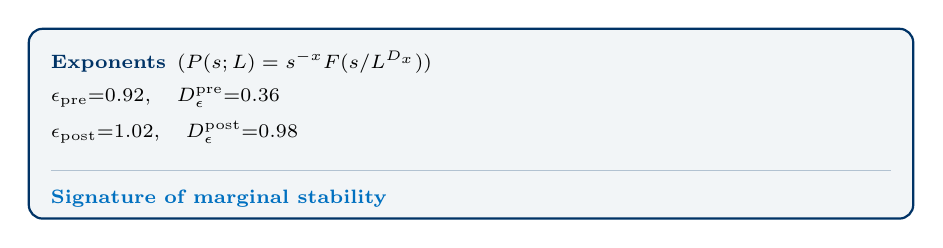
\begin{tikzpicture}
        \node[draw=AcademicNavy, thick, fill=AcademicNavy!5, rounded corners=5pt, inner sep=8pt] {
            \begin{minipage}[c][1.8cm][s]{0.88\linewidth}
                {\scriptsize \textbf{\color{AcademicNavy} Exponents}\enspace($P(s;L)=s^{-x}F(s/L^{D_x})$)}
                \vfill
                {\scriptsize
                    $\epsilon_\text{pre}{=}0.92,\quad D_\epsilon^\text{pre}{=}0.36$\\[0.03cm]
                    $\epsilon_\text{post}{=}1.02,\quad D_\epsilon^\text{post}{=}0.98$
                }
                \vfill
                \textcolor{AcademicNavy!30}{\rule{\linewidth}{0.3pt}}
                \vfill
                {\scriptsize \textbf{\color{SteelBlue} Signature of marginal stability}}
            \end{minipage}
        };
    \end{tikzpicture}
\end{columns}

\vspace{0.08cm}

% ---- Row 2: Rebonding in Action ----
\textcolor{SteelBlue}{\rule{\linewidth}{0.8pt}}\\[0.03cm]
{\small \textcolor{AcademicNavy}{\textbf{Rebonding in action}}}

\vspace{0.04cm}

\begin{center}
    \animategraphics[autoplay,loop,width=0.58\linewidth]{10}{side_by_side_frames/frame_}{001}{162}
\end{center}



\end{frame}

\end{document}
